% Created 2020-11-27 ven. 10:07
% Intended LaTeX compiler: pdflatex
\documentclass[a4paper]{article}
\usepackage[utf8]{inputenc}
\usepackage[T1]{fontenc}
\usepackage{graphicx}
\usepackage{grffile}
\usepackage{longtable}
\usepackage{wrapfig}
\usepackage{rotating}
\usepackage[normalem]{ulem}
\usepackage{amsmath}
\usepackage{textcomp}
\usepackage{amssymb}
\usepackage{capt-of}
\usepackage{natbib}
%\usepackage{subfigure}
\usepackage{subcaption}
\usepackage[linktocpage,pdfstartview=FitH,colorlinks,
linkcolor=blue,anchorcolor=blue,
citecolor=blue,filecolor=blue,menucolor=blue,urlcolor=blue]{hyperref}
\usepackage{geometry}
\geometry{a4paper,total={170mm,257mm},left=10mm,	top=20mm,	rmargin = 20mm,	bottom = 20mm}
\usepackage{babel}
\newtheorem{theorem}{Theorem}
\newtheorem{corollary}{Corollary}
\newtheorem{lemma}[theorem]{Lemma}
\newtheorem{Proposition}{Proposition}
\newtheorem{Remark}{Remark}
\newtheorem{Assumption}{Assumption}
\newtheorem{Definition}{Definition}
\usepackage{graphicx}

\def\1{{\bf 1}_N}
\def\0{{\bf 0}}
\def\N{{\mathbb N}}
\def\R{{\mathbb R}}
\def\E{\mathcal{E}}
\def\G{\mathcal{G}}
\def\T{\mathcal{T}}
\def\I{\mathcal{I}}
\def\L{\mathcal{L}}
\def\P{\mathcal{P}}
\newcommand{\unn }{\{1,\ldots, n\}}
\newcommand{\unN}{\{1,\ldots, N\}}
%\author{Bikash Adhikari}
%\date{\today}
\title{Report: Synthesis of optimal filter for MHOQ} 
%\hypersetup{
% pdfauthor={Bikash Adhikari},
% pdftitle={Linear Quadratic Regulator (LQR)},
% pdfkeywords={},
% pdfsubject={},
% pdfcreator={Emacs 26.3 (Org mode 9.3.6)}, 
% pdflang={English}}


\begin{document}
\newpage
\maketitle
\tableofcontents

\section{Quantisation}
Let $w \in \mathbb{R}$ be the input, $\mathbf{Q}$ be the quantiser and $y \in \mathbb{U}$ the quantiser output, as shown in the additive model of quantisation in the Figure \ref{fig:quan_add_model}.  Let us define the quantisation error as 
\begin{equation}
	q = \mathbf{Q}(w) - w= y -w.
	\label{eq:error}
\end{equation}
\begin{figure}
    \centering
    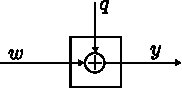
\includegraphics[scale = 1]{figures/quantizer_additive_model.pdf}
    \caption{Quantiser additive model}
    \label{fig:quan_add_model}
\end{figure}
The quantisation requires the signal to be mapped to a finite signal where each value of the output $y$ is restriced to belong to a finite set $\mathbb{U}$. The elements of the set $\mathbb{U}$ represent the quantiser levels and depends on the word-size of the quantiser. 

\section{Noise shaping quantiser}
Noise-shaping quantisers can reduce the effective quantisation error by moving quantisation noise to higher 
frequencies through oversampling and feedback.  The reconstruction filter is then used to attenuate the 
frequency-shaped quantisation noise. It operates by estimating the uniform quantisation error and employing a 
feedback filter to shape the noise power at the output of the DAC. A block diagram for a noise-shaping quantiser 
is shown in Fig. \ref{fig:dsm1}. The feedback filter $F(z)$ is designed such that the transfer 
function $y = (1 - F(z)) \epsilon$ is a high-pass filter.

\begin{figure}[!h]
	\centering
	\begin{minipage}{0.45\linewidth}
		\centering
		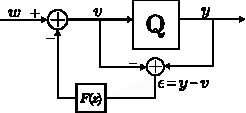
\includegraphics[scale = 1.5]{figures/noise_shaping2.pdf}
		\caption{Noise shaping quantiser}
		\label{fig:dsm}
	\end{minipage}
	\hfil  
	\begin{minipage}{0.45\linewidth}
		\centering
		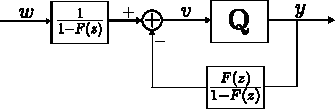
\includegraphics[scale = 1.5]{figures/noise_shaping_redrawn.pdf}
		\caption{Noise shaping quantiser}
		\label{fig:dsm1}
	\end{minipage}
\end{figure}



In linear analysis, the output is given by 
\begin{equation}
	Y(z) = \textbf{STF}. W(z) + \textbf{NTF} .E(Z)
\end{equation}
where the signal transfer function $\textbf{STF} = 1$, noise transfer function $\textbf{NTF} =  (1-F)$ with $F$ being a noise shaping filter. $F = z^{-1}$ is the special case known as 
the first-order delta-sigma modulator. 

\section{Moving horizon optimal quantiser (MHOQ)}
The design criteria for the MHOQ is the minimization of the perceived errors defined as follows:
\begin{equation}
	e(t) = H(z)(w(t)-y(t))
	\label{eq:error1}
\end{equation}
where  $H(z)$  is  a stable time-invariant linear low-pass filter with the following state-space
\begin{equation}
	\label{eq:filter_statespace}
	H(z) = 1 + C(z I - A)^{-1} B
\end{equation}
The error $e$  then can be written as the output of the following state-space representation of $H$
\begin{equation}
	\begin{aligned}
		x(t+1) &= A x(t) + B (w(t)-y(t))		\\
		e(t) &= Cx(t) + w(t)-y(t)
	\end{aligned}
	\label{eq:statespace1}
\end{equation}
where $x \in \mathbb{R}^{n}$ is the state vector.  The error $e$ corresponds to the difference between the filtered quantised signal and the filtered input signal. 

For moving horison implementation, the optimisation problem is defined as the problem of finding $y \in \mathbb{U}$ that minimises  the cost function  while satisfying the state equations as follows:
\begin{align}
		& y^{\ast}(t) = \arg  \min_{y(t) }	V_{N}  = \sum_{t=k}^{k+N-1} e^{2}(t) \label{eq:optobj1}\\
		\intertext{subject to}
		&x(t+1) = A x(t) + B (w(t)-y(t))	\label{eq:optconst1}	\\
		&e(t) = Cx(t) + w(t)-y(t)	\label{eq:optconst2}	\\
		&y(t) \in \mathbb{U}. \label{eq:optconst3}
	\end{align}
\subsection{Alternative binary formulation}
The optimization problem \eqref{eq:optobj1}-\eqref{eq:optconst3} can be reformulated as an optimization problem with the binary variables. Let $\mathcal{B}$ be the number of bits.  $b_{i} = \{0,1\}$ and $Q_{i}$ $, i = \{0, 1, \ldots, 2^{\mathcal{B}}-1\}$, be the binary variables and quantisation levels, respectively. 
\begin{align}
		& y^{\ast}(t) = \arg  \min_{y(t) }	V_{N}  = \sum_{t=k}^{k+N-1} e^{2}(t) \label{eq:optobj12}\\
		\intertext{subject to}
		&x(t+1) = A x(t) + B (w(t)-y(t))	\label{eq:optconst12}	\\
		&e(t) = Cx(t) + (w(t)-y(t))	\label{eq:optconst22}	\\
		&y(t) = \sum_{i = 0}^{2^{\mathcal{B}}-1} Q_{i}b_{i}, \quad \sum_{i = 0}^{2^{\mathcal{B}}-1}b_{i}  =1, \quad b_{i} = \{0,1\}. \label{eq:optconst32} 
	\end{align}

% \section{Frequency response: LPF and NTF}
% \subsection{Perception filter}
% The  frequency response and the STF and NTF of the perception filter used in  
% \cite{goodwin2003moving} are shown in the
% figure below, 
% \begin{figure}[!h]
% 	\centering
% \begin{minipage}{0.45\linewidth}
% 	\centering
% 	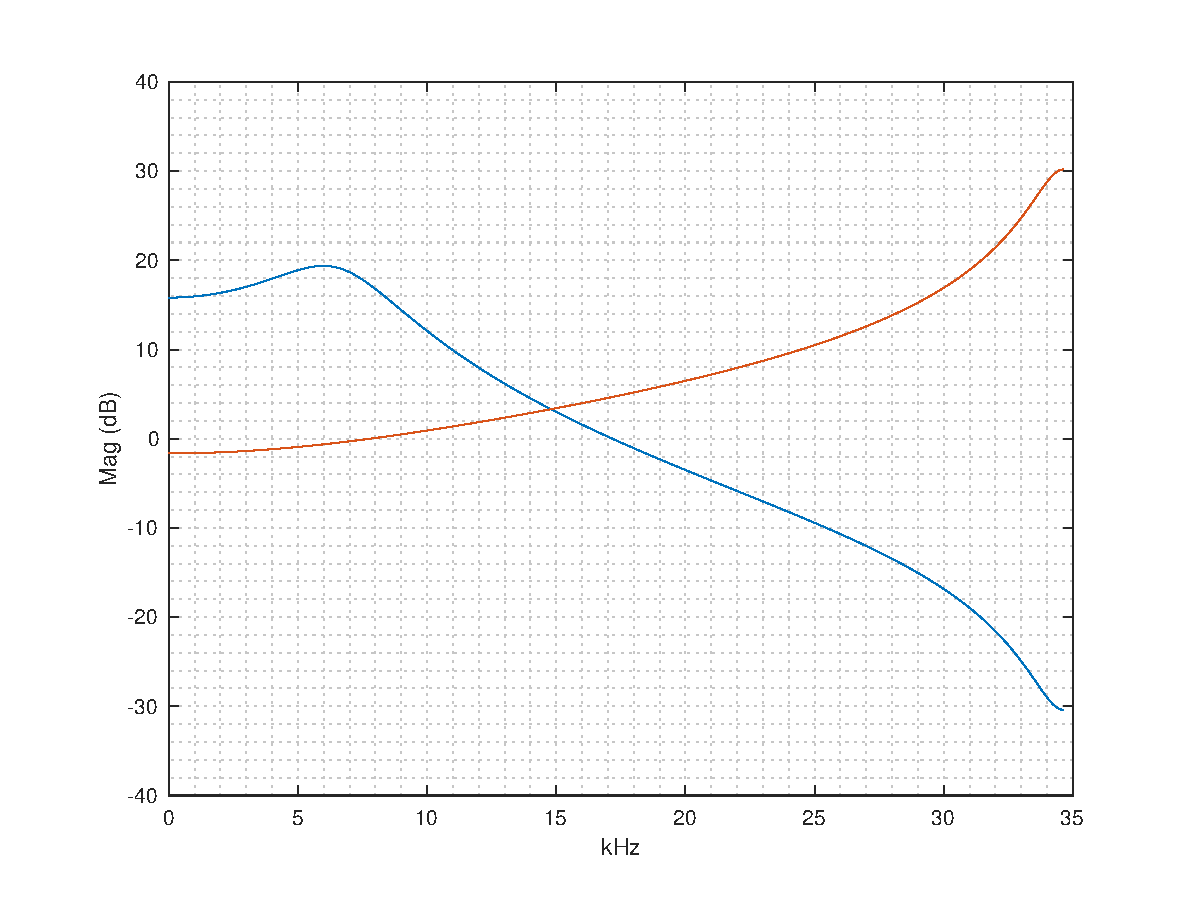
\includegraphics[scale = 0.45]{plots/percp.eps}
%         \caption{Perception filter Frequency response}
% 	\end{minipage}
% 	\hfil
% 	\begin{minipage}{0.45\linewidth}
% 	\centering
% 	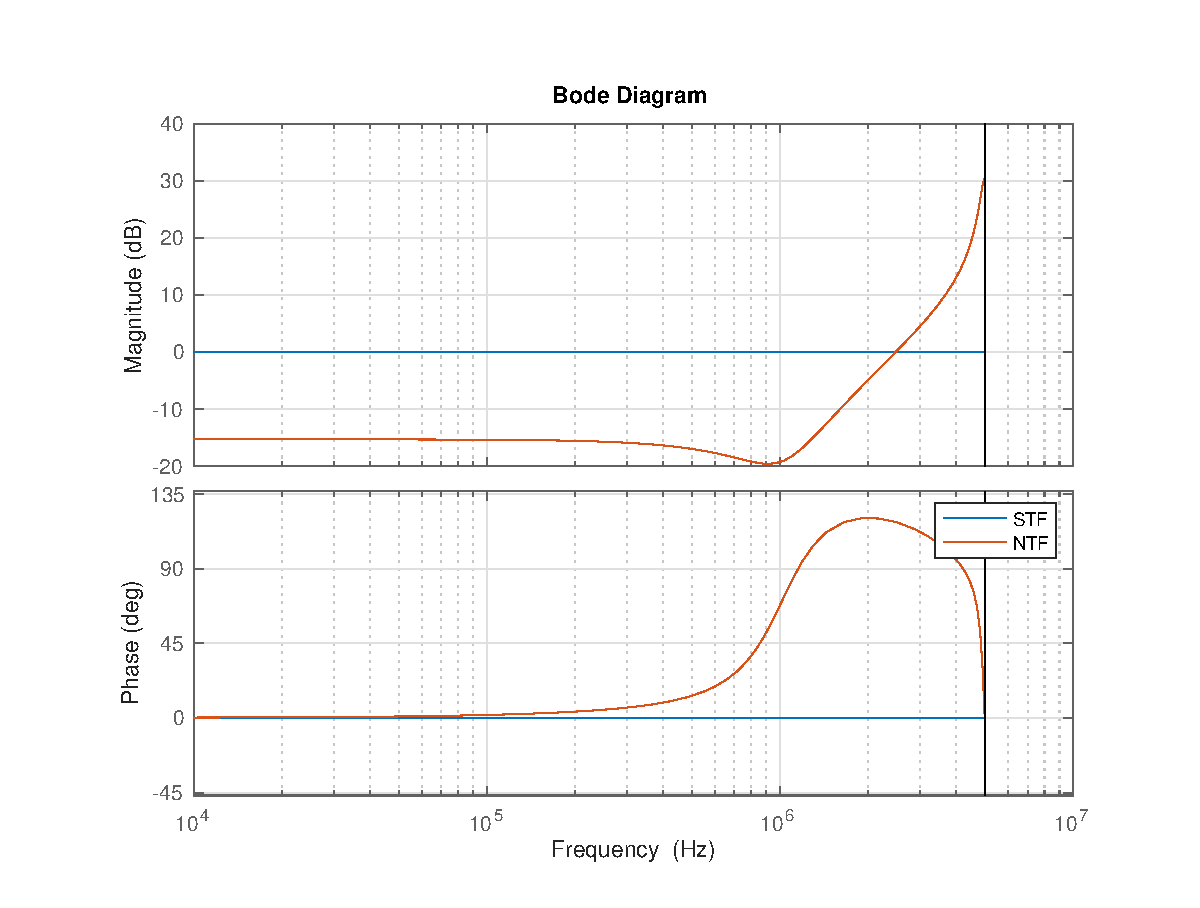
\includegraphics[scale = 0.45]{plots/stf_ntf_perception_linear.eps}
% 		\caption{STF and NTF using perception filter}
% \end{minipage}
% \end{figure}


% \subsection{Butterworth Filter}

% \begin{figure}[!h]
% 	\centering
% 	\begin{minipage}{0.45\linewidth}
% 		\centering
% 		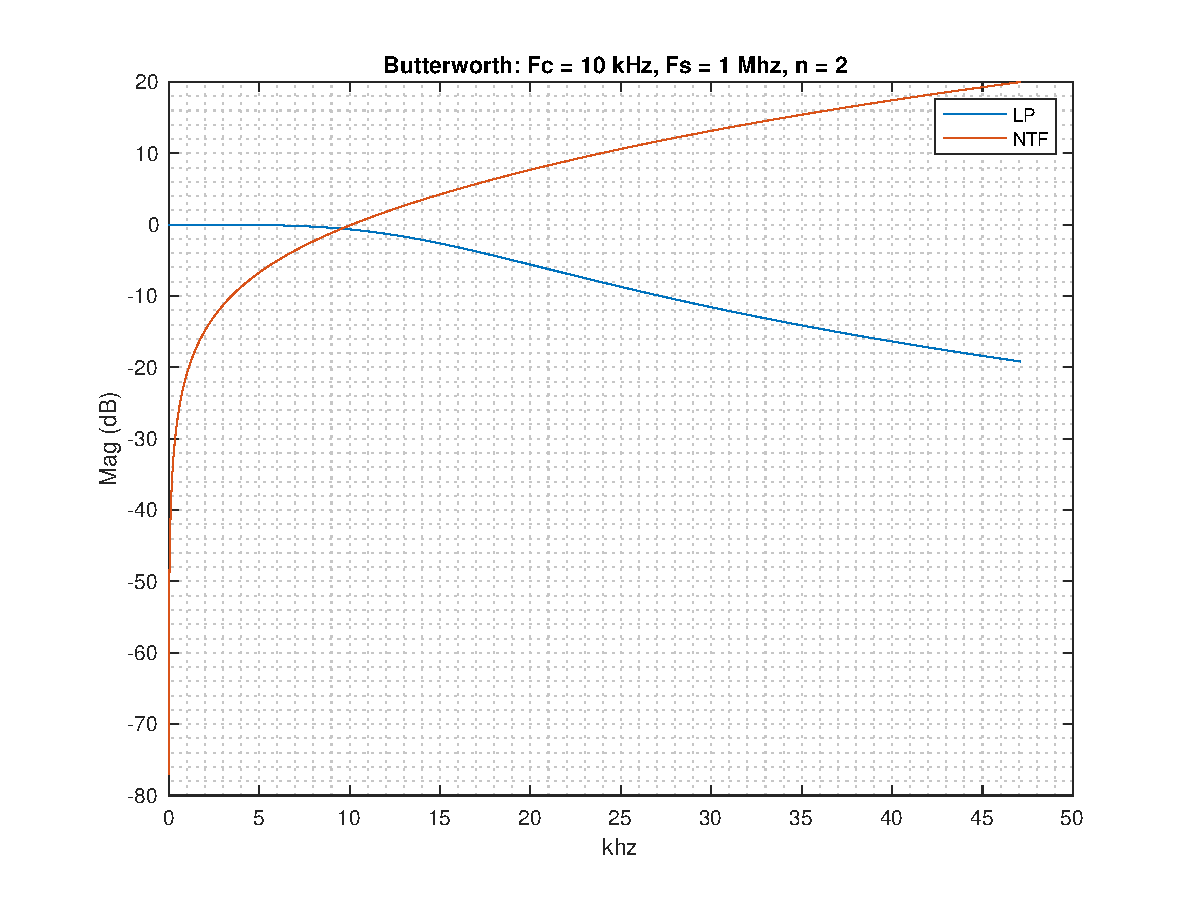
\includegraphics[scale = 0.45]{plots/but_lp_ntf_2_10.eps}
% 		\caption{Frequency response of low-pass Butterworth and  corresponding high-pass  NTF}
% 	\end{minipage}
% 	\hfil
% 	\begin{minipage}{0.45\linewidth}
% 		\centering
% 		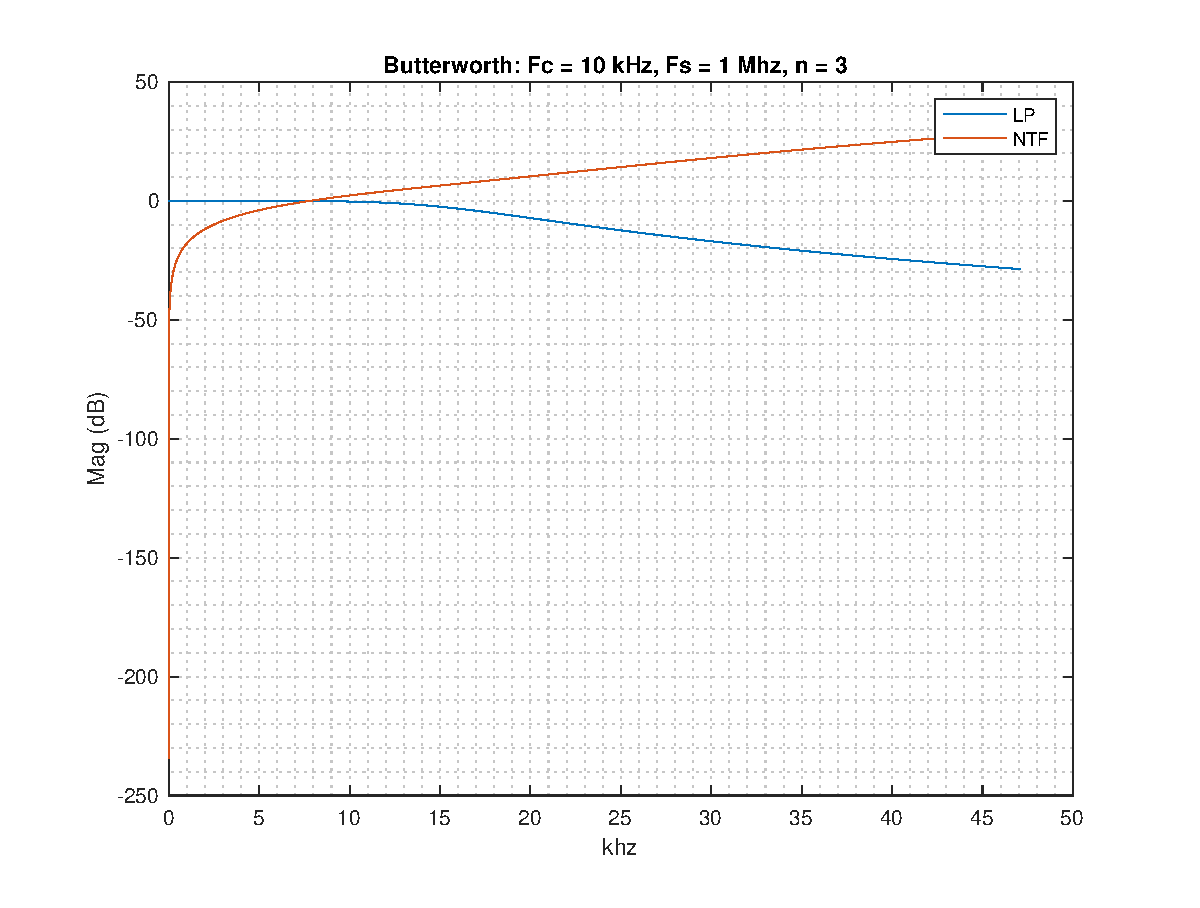
\includegraphics[scale = 0.45]{plots/but_lp_ntf_3_10.eps}
% 		\caption{Frequency response of low-pass Butterworth and  corresponding high-pass  NTF}
% 	\end{minipage}
% \end{figure}

% \begin{figure}[!h]
% 	\centering
% 	\begin{minipage}{0.45\linewidth}
% 		\centering
% 		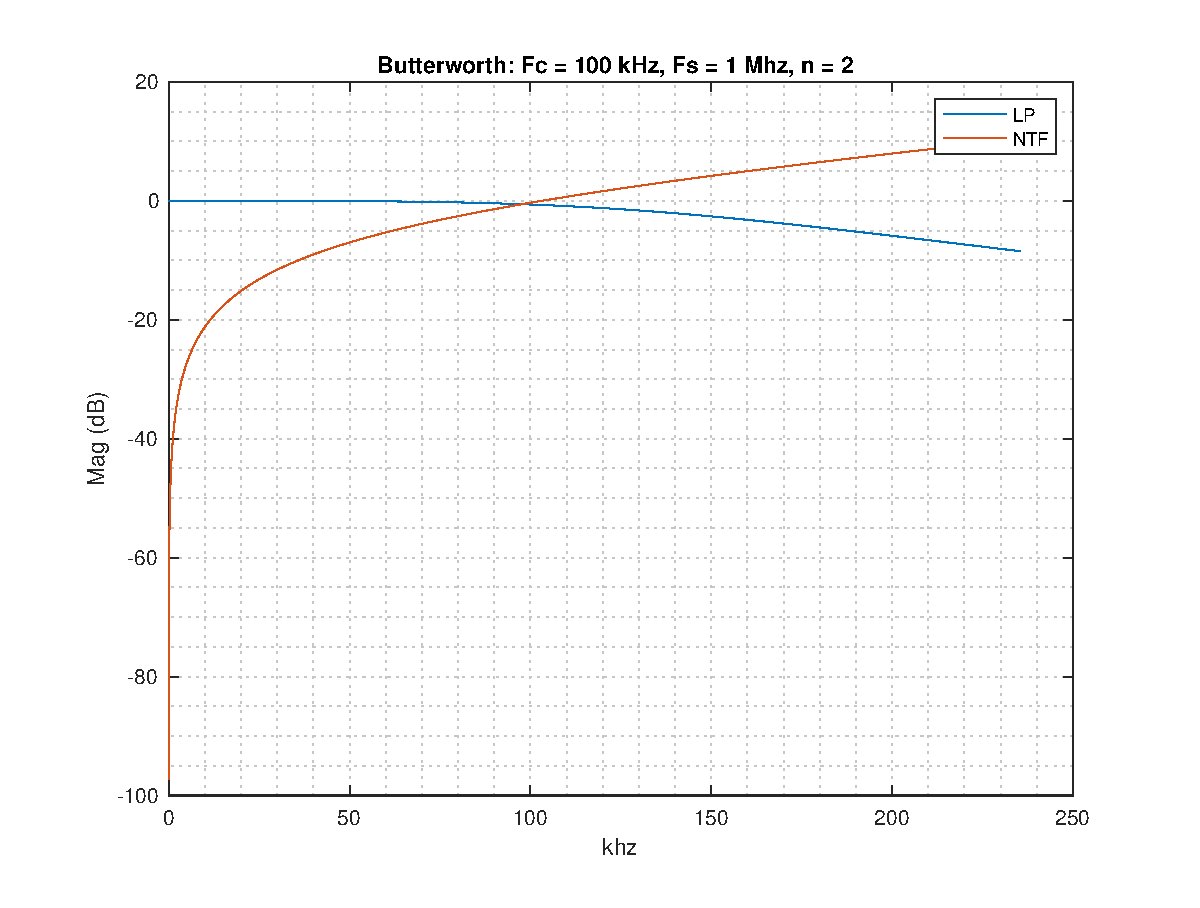
\includegraphics[scale = 0.45]{plots/but_lp_ntf_2_100_1000.eps}
% 		\caption{Frequency response of low-pass Butterworth and  corresponding high-pass  NTF}
% 	\end{minipage}
% 	\hfil
% 	\begin{minipage}{0.45\linewidth}
% 		\centering
% 		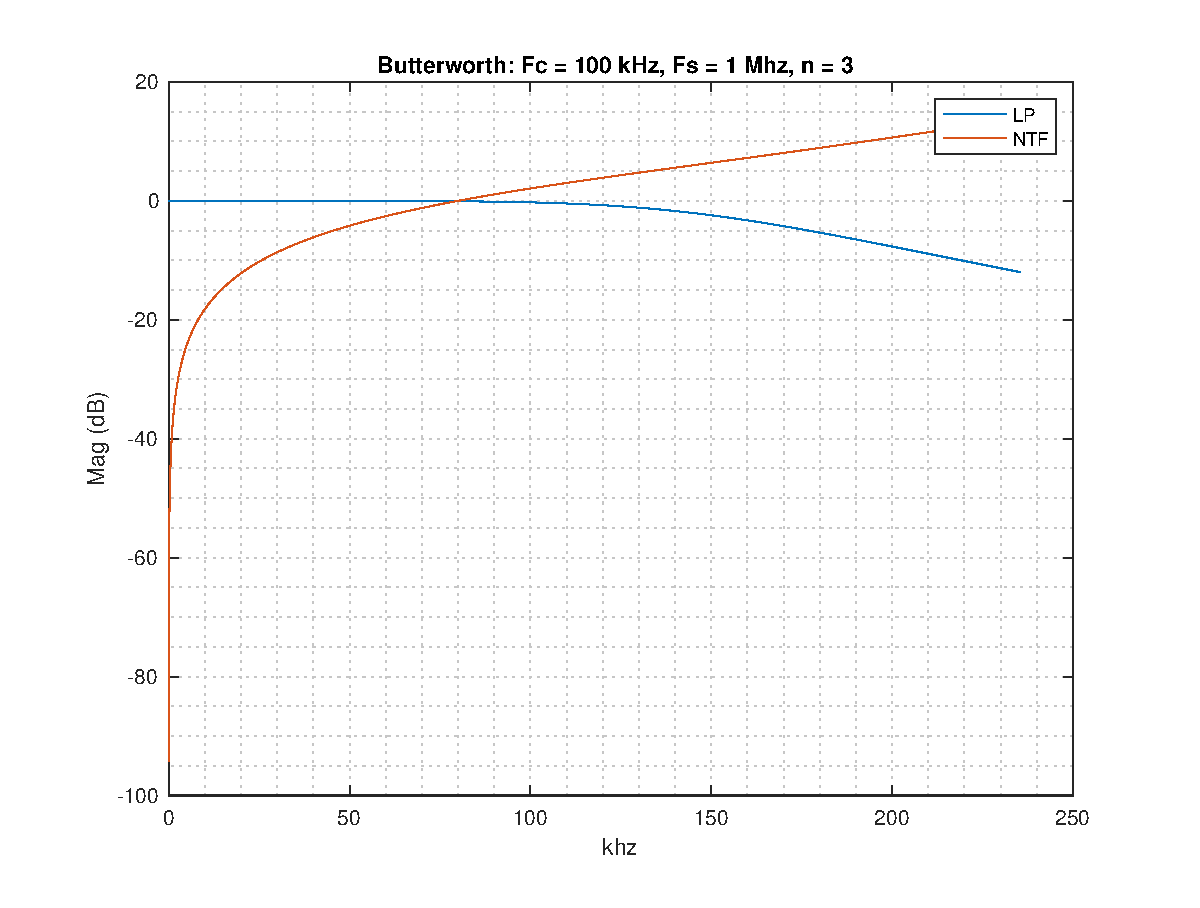
\includegraphics[scale = 0.45]{plots/but_lp_ntf_3_100_1000.eps}
% 		\caption{Frequency response of low-pass Butterworth and  corresponding high-pass  NTF}
% 	\end{minipage}
% \end{figure}


\section{Noise Transfer Function(NTF)}
The frequency response of the noise transfer functions due to butterworth filters at different cutoff frequencies are shown in the figure Fig. \ref{fig:NTFvsfreq}. In the figure, we can see that the net area under the curve remain the same.   In Fig. \ref{fig:LPFNTFvsfreq} the frequency reponse of the low pass filter is plotted along with that of the noise transefer function. This observation shows that the better performance can be achieved by increasing the cutoff frequency during MHOQ while keeping the cutoff frequency of the reconstruction as same. The simulation results in the following table confirm this observation. 

\begin{table}[!h]
	\caption{ENOB at different cutoff frequencies. Reconstruction filter: Butterworth LPF with $n =2$,  $Fc = 100 \textrm{kHz}$ and $Fs = 1\textrm{Mhz}$.}
	\centering
	\begin{tabular}{|c|c|c|c|c|c|}
	\hline
	Fc & 100 kHz & 200 kHz & 300 kHz & 400 kHz & 500 kHz \\
	\hline
	ENOB & 3.981 & 5.307 & 7.817  & 10.481 & 10.936\\
	\hline
	\end{tabular}	
	
\end{table}

\begin{figure}[!h]
	\centering
	\begin{minipage}{0.45\linewidth}
		\centering	
		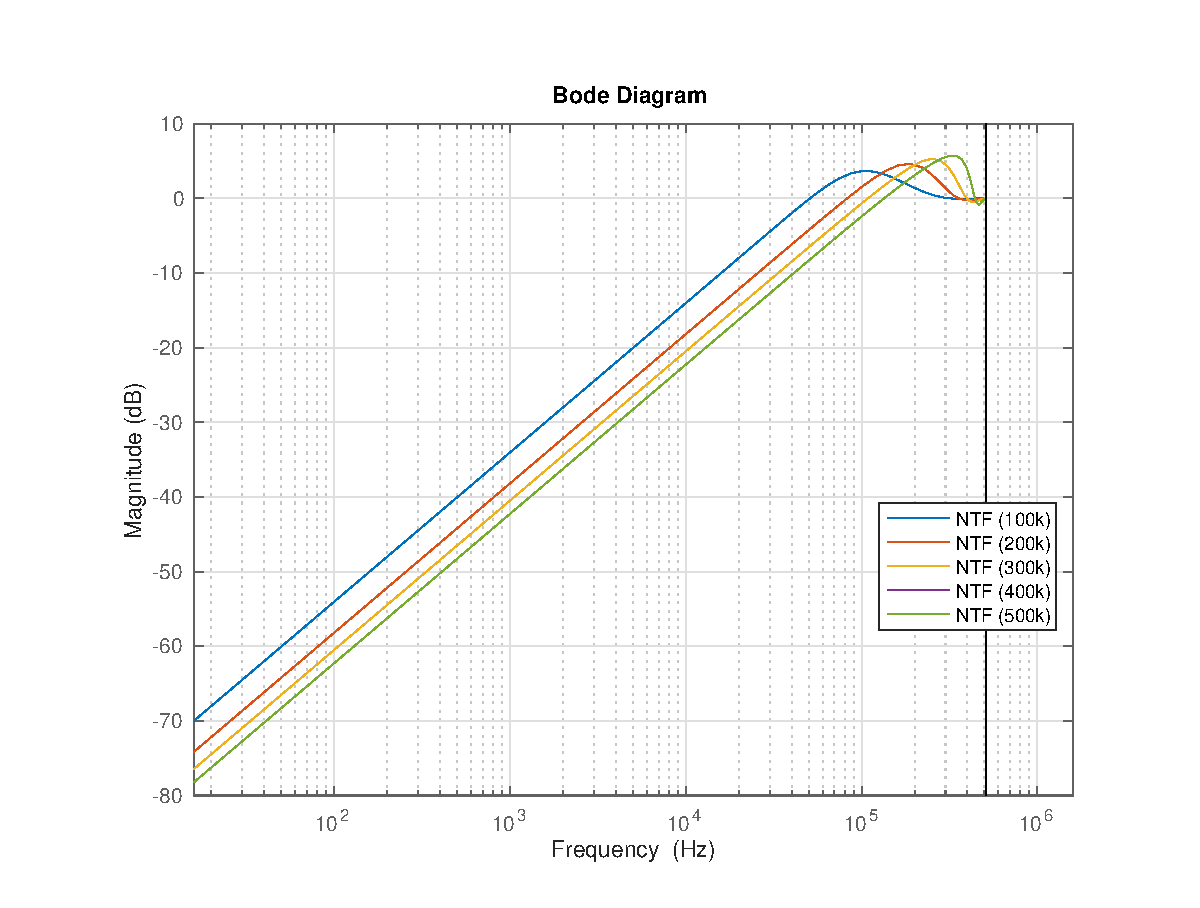
\includegraphics[scale = 0.5]{fig_stf_ntf/ntf_vs_freq.eps}
		\caption{Frequency response of NTF for different cutoff frequency}
		\label{fig:NTFvsfreq}
	\end{minipage}
	\hfil
	\begin{minipage}{0.45\linewidth}
		\centering
		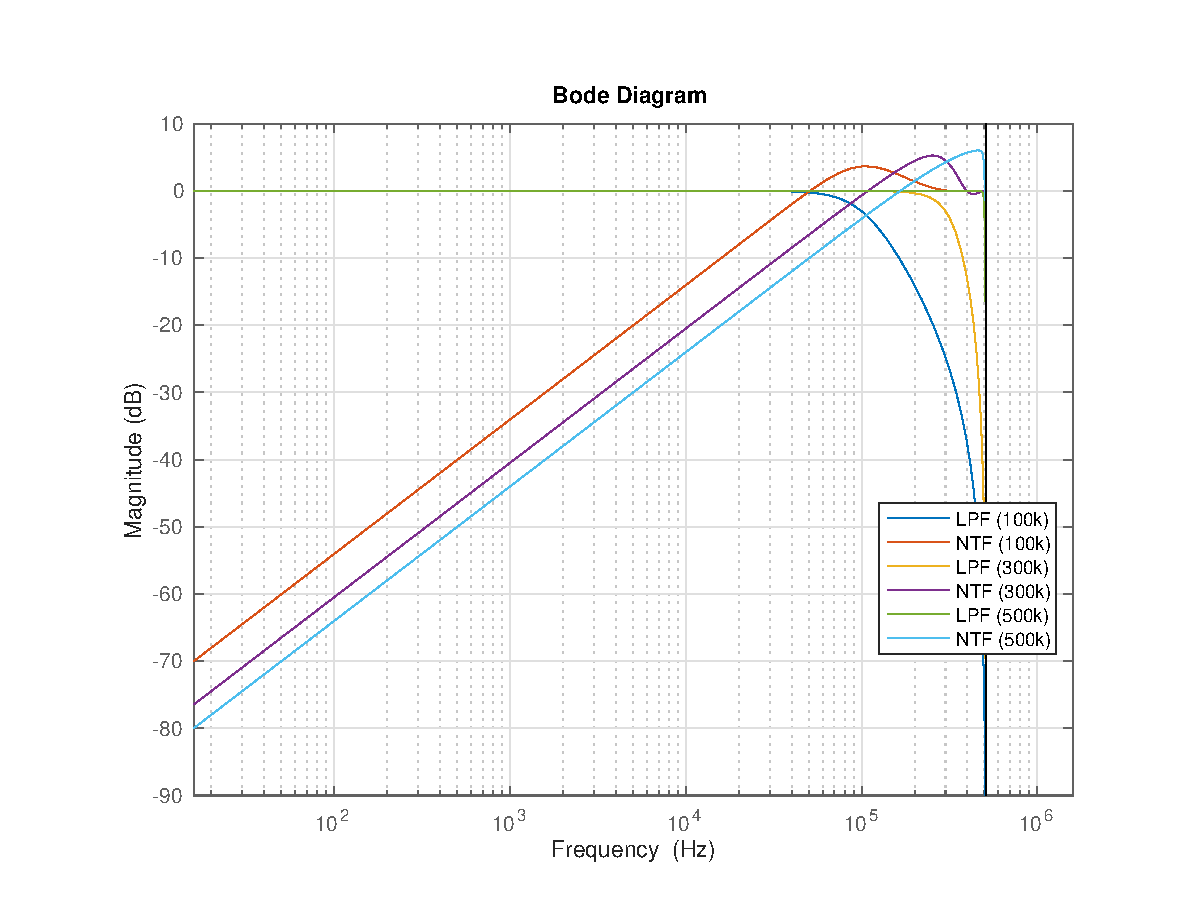
\includegraphics[scale = 0.5]{fig_stf_ntf/lpf_ntf_vs_freq.eps}
		\caption{Frequency response of LPF and NTF for different cutoff frequency}
		\label{fig:LPFNTFvsfreq}
	\end{minipage}
\end{figure}


% \begin{figure}[!h]
% 	\centering
% 	\begin{minipage}{0.45\linewidth}
% 		\centering
% 		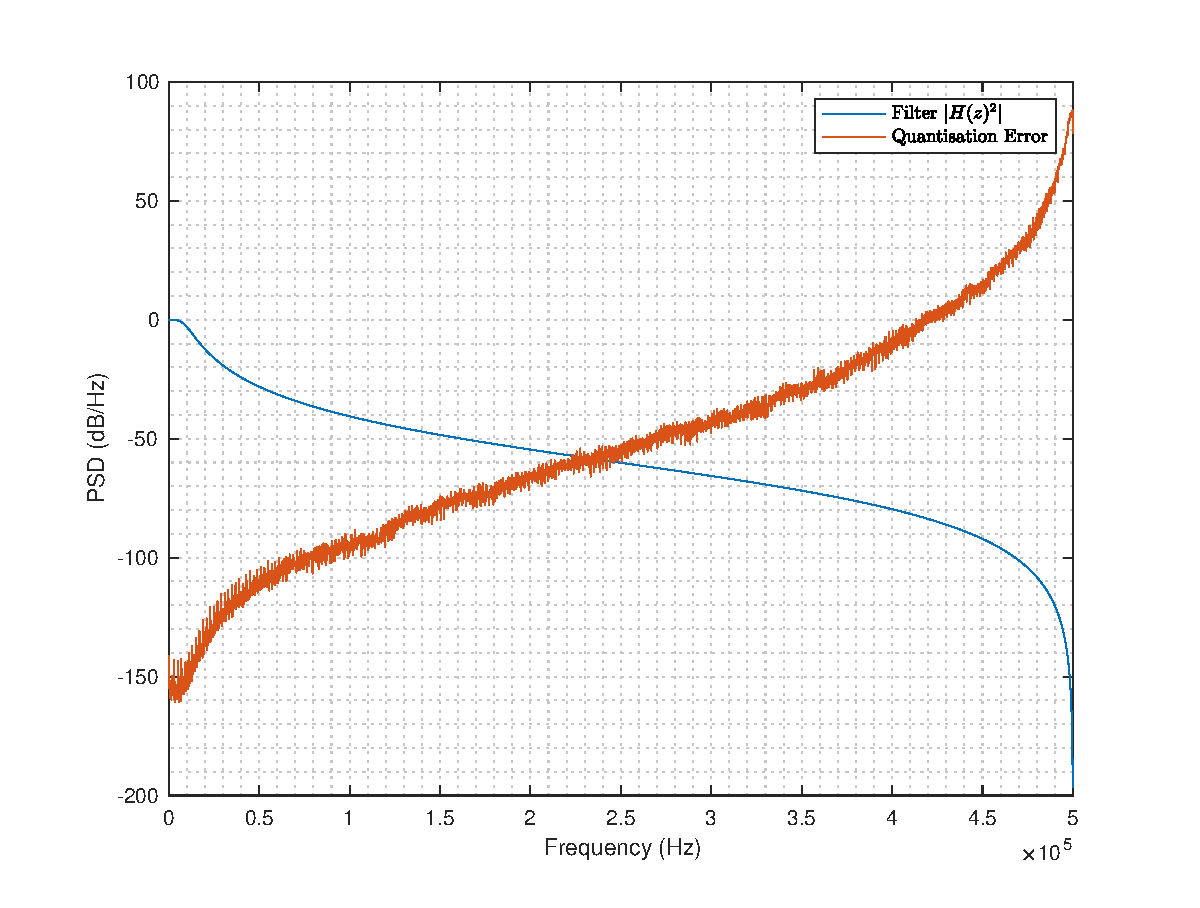
\includegraphics[scale = 0.45]{plots/quant_err_butter_2nd_10k_1mhz_inl.eps}
% 		\caption{Butterworth Frequency response and frequency spectrum of quantisation noise:  
% 				\\ \textbf{Fc} = 10 kHz, \textbf{Fs} = 1 MHz, \textbf{ENOB} = 18.47, \textbf{Uniform}}
% 	\end{minipage}
% 	\hfil
% 	\begin{minipage}{0.45\linewidth}
% 		\centering
% 		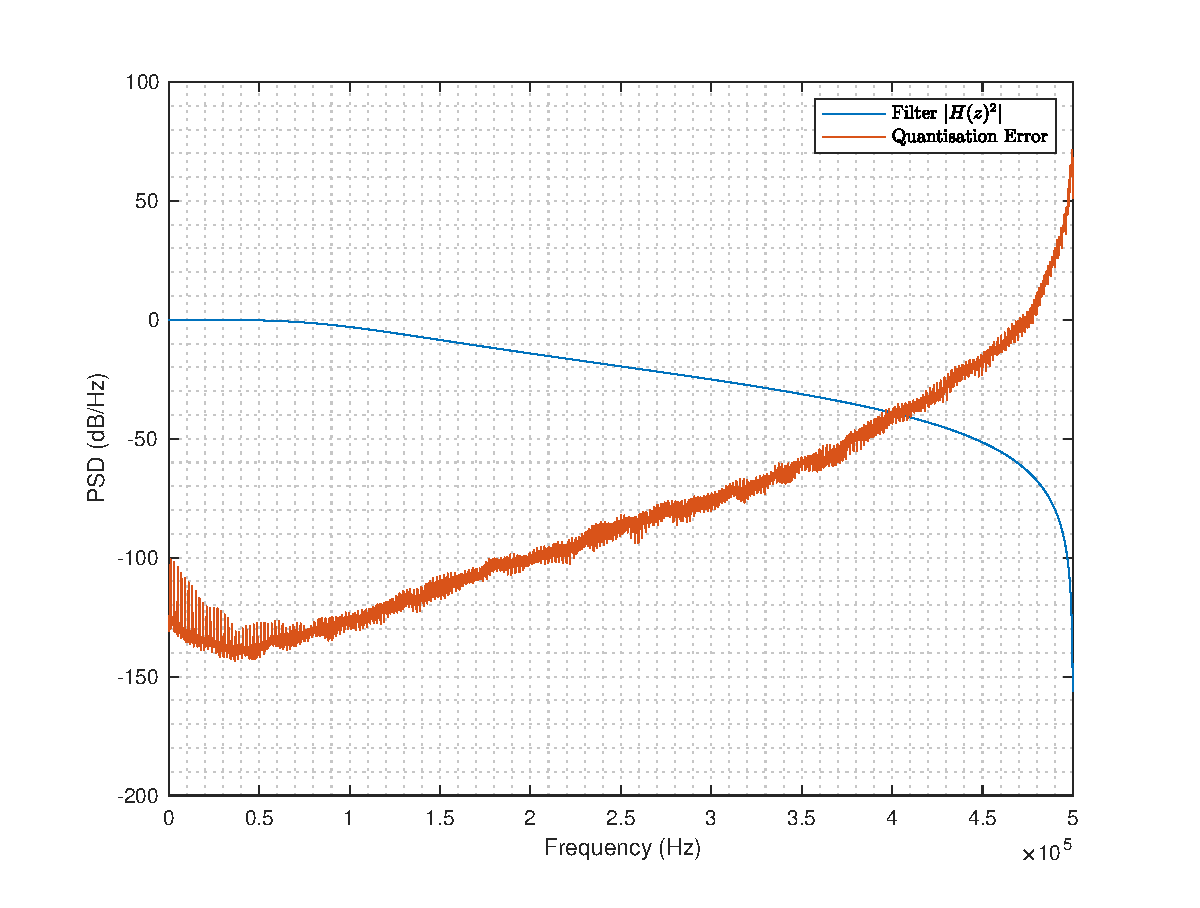
\includegraphics[scale = 0.45]{plots/quant_err_butter_2nd_100k_1mhz_ideal.eps}
% 		\textbf{\caption{Butterworth Frequency response  and frequency spectrum of quantisation noise:  
% 					\\ \textbf{Fc} = 100 kHz, \textbf{Fs} = 1 MHz, \textbf{ENOB} = 9.09, \textbf{Uniform}
% 				}}
% 	\end{minipage}
% \end{figure}

% \begin{figure}[!h]
% 	\centering
% 	\begin{minipage}{0.45\linewidth}
% 		\centering
% 		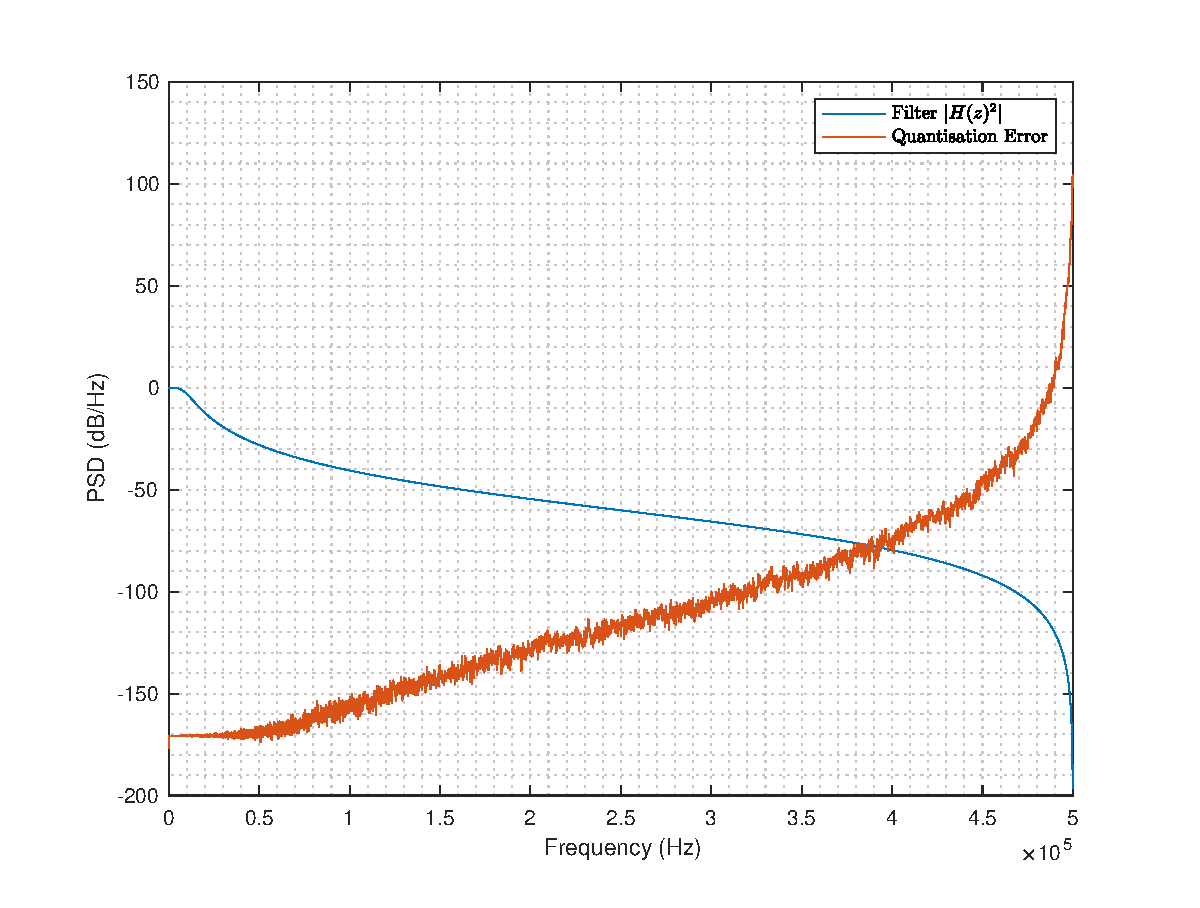
\includegraphics[scale = 0.45]{plots/filt_vs_qnoise_10k_fs10mhz_ideal.eps}
% 		\caption{Butterworth Frequency response and frequency spectrum of quantisation noise:  
% 				\\ \textbf{Fc} = 10 kHz, \textbf{Fs} = 10 MHz, \textbf{ENOB} = 26.2, \textbf{Uniform}
% }
% 	\end{minipage}
% 	\hfil
% 	\begin{minipage}{0.45\linewidth}
% 		\centering
% 		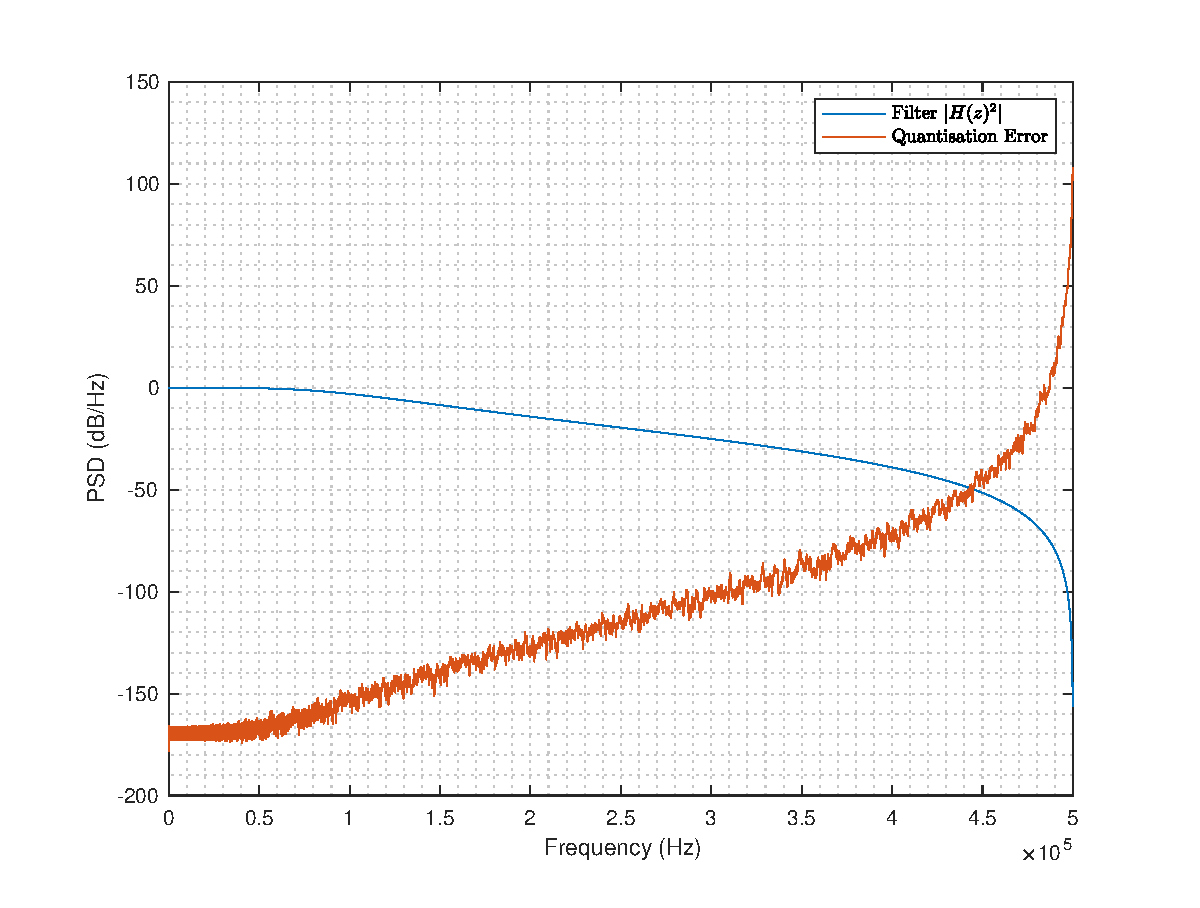
\includegraphics[scale = 0.45]{plots/filt_vs_qnoise_100k_fs10mhz_ideal.eps}
% 		\textbf{\caption{Butterworth Frequency response  and frequency spectrum of quantisation noise: 
% 					\\ \textbf{Fc} = 100 kHz, \textbf{Fs} = 10 MHz, \textbf{ENOB} = 17.31, \textbf{Unifrom}
% }}
% 	\end{minipage}
% \end{figure}
\newpage
\section{Spectrum of quantisation noise}
The sampling frequency effects the spectrum of the quantisation noise and consequently the ENOB as shown in the following figures. 

\begin{figure}[!h]
	\centering
	\begin{minipage}{0.45\linewidth}
		\centering
		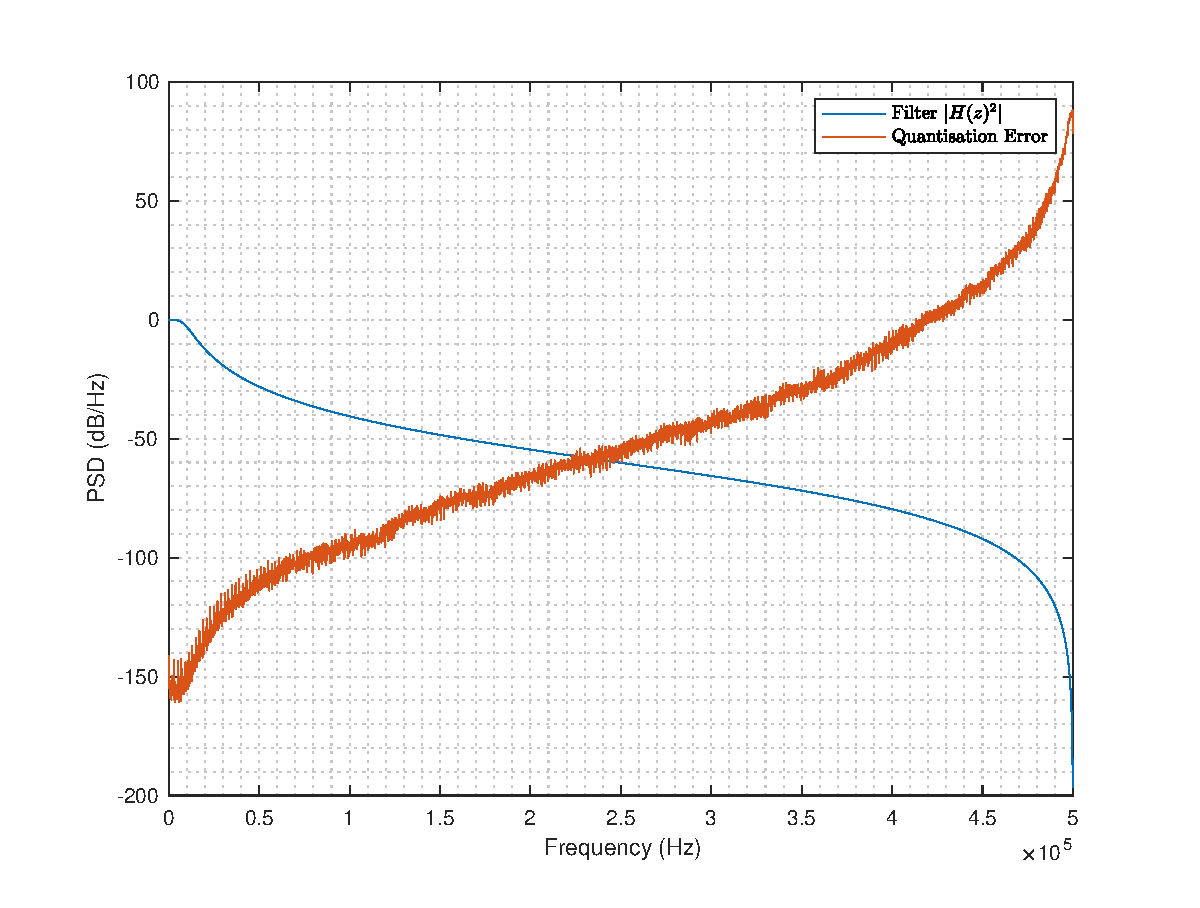
\includegraphics[scale = 0.45]{plots/quant_err_butter_2nd_10k_1mhz_inl.eps}
		\caption{Butterworth Frequency response and frequency spectrum of quantisation noise:  
			\\ \textbf{Fc} = 10 kHz, \textbf{Fs} = 1 MHz, \textbf{ENOB} = 16.58, \textbf{INL} }
	\end{minipage}
	\hfil
	\begin{minipage}{0.45\linewidth}
		\centering
		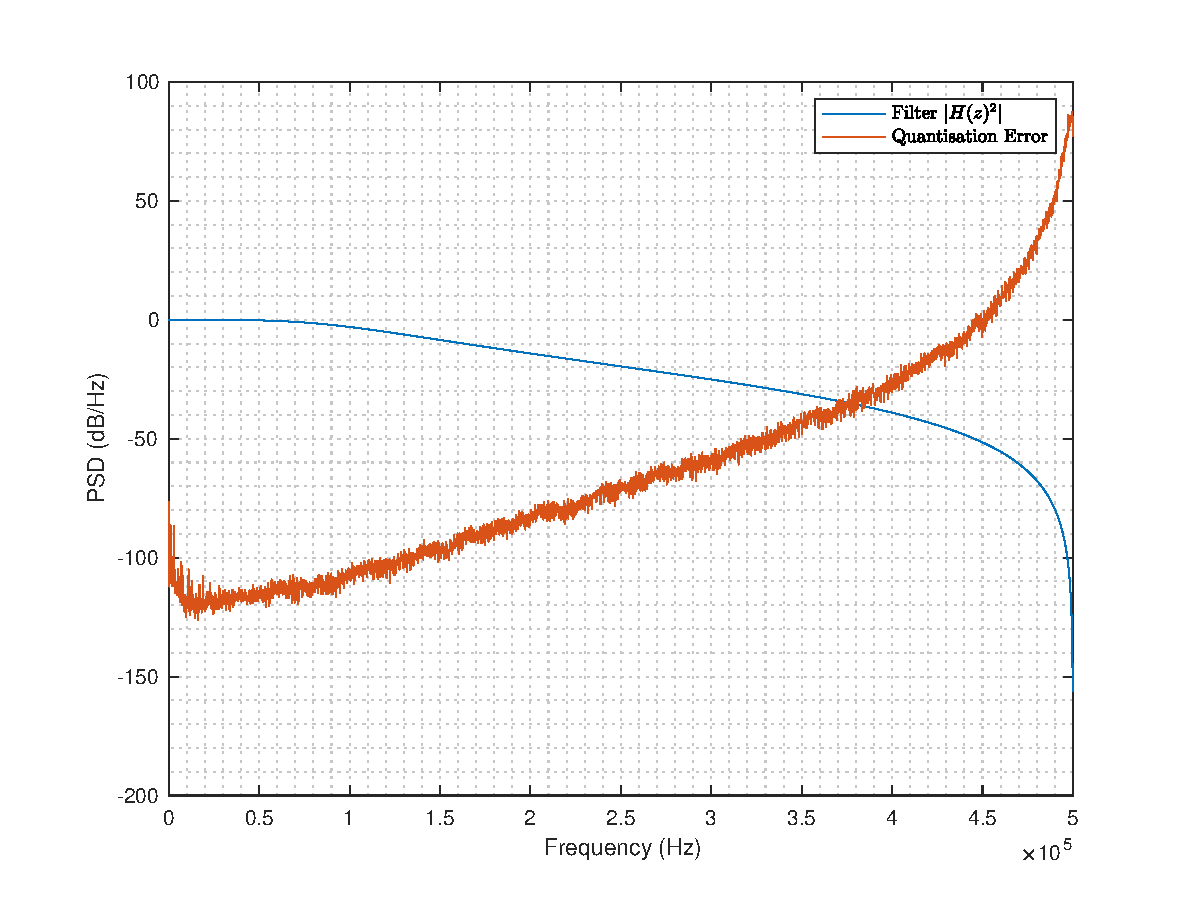
\includegraphics[scale = 0.45]{plots/quant_err_butter_2nd_100k_1mhz_inl.eps}
		\textbf{\caption{Butterworth Frequency response  and frequency spectrum of quantisation noise: 
					\\ \textbf{Fc} = 100 kHz, \textbf{Fs} = 1 MHz, \textbf{ENOB} =7.43, \textbf{INL}
 }}
	\end{minipage}
\end{figure}

\begin{figure}[!h]
	\centering
	\begin{minipage}{0.45\linewidth}
		\centering
		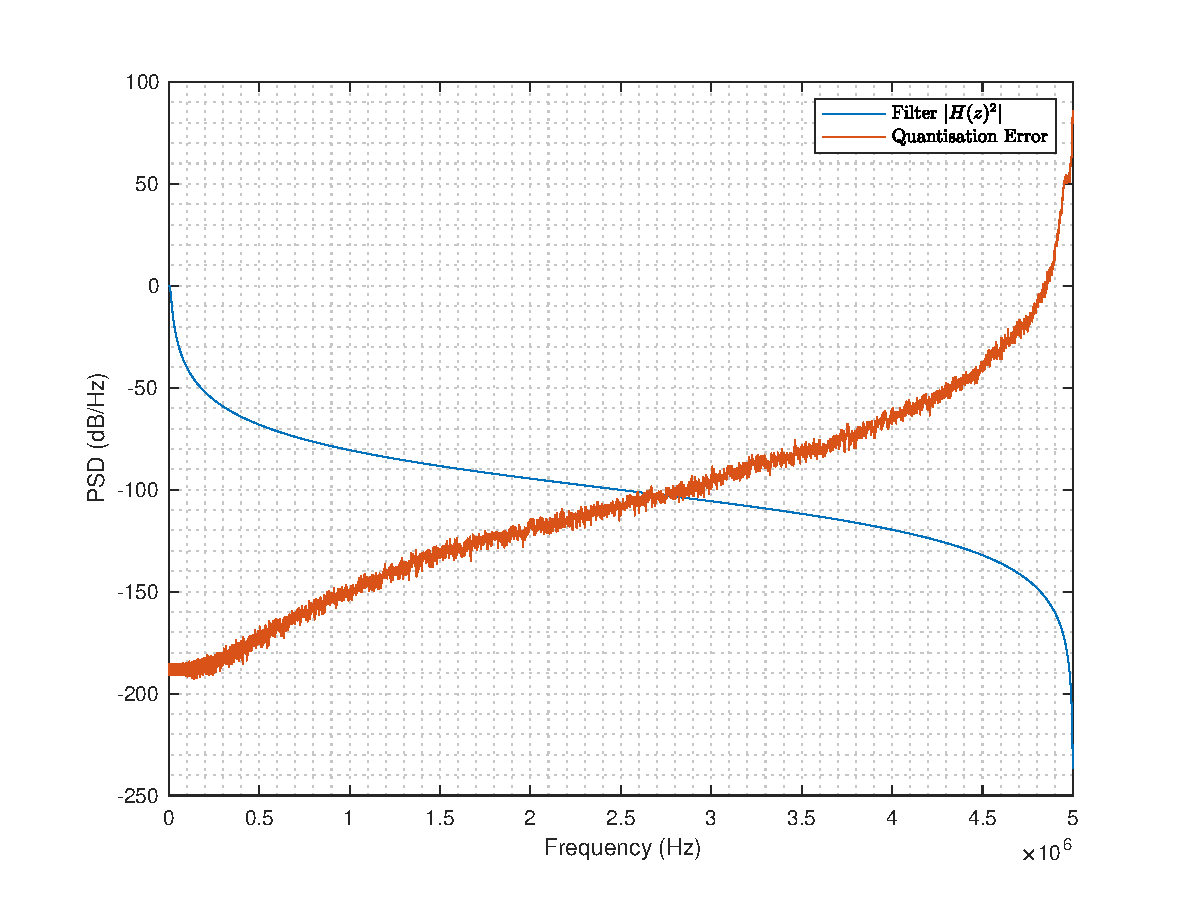
\includegraphics[scale = 0.45]{plots/quant_err_butter_2nd_10k_10mhz_inl.eps}
		\caption{Butterworth Frequency response and frequency spectrum of quantisation noise: 
		\\ \textbf{Fc} = 10 kHz, \textbf{Fs} = 10 MHz, \textbf{ENOB} = 25.12, \textbf{INL}}
	\end{minipage}
	\hfil
	\begin{minipage}{0.45\linewidth}
		\centering
		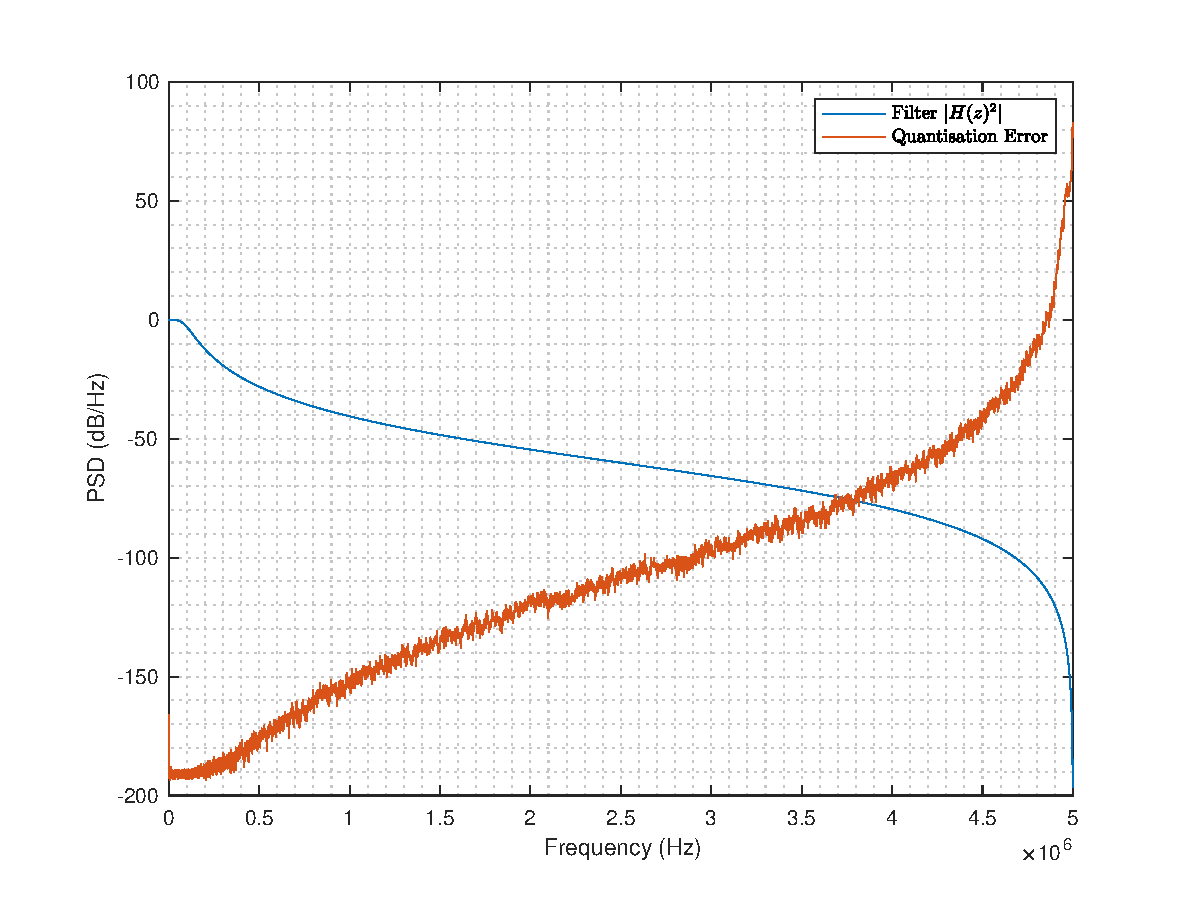
\includegraphics[scale = 0.45]{plots/quant_err_butter_2nd_100k_10mhz_inl.eps}
		\textbf{\caption{Butterworth Frequency response  and frequency spectrum of quantisation noise:  
			\\ \textbf{Fc} = 100 kHz, \textbf{Fs} = 10 MHz, \textbf{ENOB} = 17.03, \textbf{INL}	
 }}
	\end{minipage}
\end{figure}

\newpage
\section{Synthesis of optimal noise-shaping filter}

\begin{figure}[!h]
	\centering
	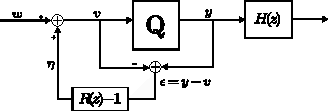
\includegraphics[scale = 2]{figures/nsq_error_feedback.pdf}
	\caption{Noise shaping quantiser and a filter $H(z)$.}
	\label{fig:nsq_efs}
\end{figure}
In noise shaping quantiser with error-feedback structure as shown in the Figure \ref{fig:nsq_efs}, the input to the quantiser is  $v = w + \eta = w + (R(z)-1)\epsilon$
and  feedback error $\epsilon$ is 
\begin{equation}
	\epsilon = y - v = y - w - (R(z)-1)\epsilon.
\end{equation}

Then quantisaion noise defined as $q := y - w$ can be expressed as 
\begin{equation}
	 q = y - w = R(z) \epsilon.
\end{equation}
Then the effect of the quantisation error on the system $H(z)$ can be expressed as 
\begin{equation}	
	 e = H(z) R(z) \epsilon.
	 \label{eq:err_plant}
\end{equation}
and it shows that we can reduce the error in the plant output by properly designing the noise shaping filter $R(z)$ with the knowledge of the plant $H(z)$. 

The objective is to design stable noise-shaping filter such that it minimises the effect of the quantisation noise in the plant output. A constraint on the error feedback signal should be imposed to prevent the quantiser from overloading and achieve a stable noise-shaping quantiser as $$ \eta = (R(z) - 1) \epsilon.$$

\begin{itemize}
	\item \textbf{Design Problem:} For a fixed pair (p,q) \cite{Shuichi2017}, 
	\begin{equation}
		\begin{aligned}
			&\min_{R(z) \in \mathbb{RH}_{\infty}} \| e \|_{p}  \\
			\textrm{subject  to.}& \\
			& R(\infty)	 = 1, \\
			& \|\eta\|_{q} < \gamma_{\eta}
		\end{aligned}	
	\end{equation}	
	where $\mathbb{RH}_{\infty} = \mathbb{R} \cap \mathbb{H}_{\infty}$ is the set of proper stable rational transfer functions.
\end{itemize}

\subsection{Solution 1: Optimal noise shaping filter without constraint}
The optimal noise shaping filter without constraint on the error feedback signal $\eta$ is the scaled inverse of the system $H(z)$.   If the quantisation error is assumed to be an i.i.d random variable with zero mean, then the variance of the error $e$ at time $k$  can be expressed as 
\begin{equation}
	E\{|e_{k}|^2\} = \|H(z) R(z) \|_{2}^{2} \sigma_{\epsilon}^{2}
\end{equation}
where $E\{.\}$ is the expectation operator and $\sigma_{\epsilon}$ is variance of the $\epsilon$ and $\|H(z) R(z) \|_{2}^{2}$  is the $\mathbb{H}_{2}$-norm.

It is shown in \cite{oppenheim99}, any casual and stable rational sytem function $H(z)$ can always be stated as the product of the minimum phase system $H_{min}(z)$ and all pass system $H_{ap}(z)$. Then it is shown that the optimal noise shaping filter is given by the scaled inverse of the plant, as follows, 
\begin{equation}
	R(z) = h_{D} H_{min}^{-1}(z)
\end{equation}
where $h_{D}$ is the first non-zero entry of the impulse response of the plant $H_{z}$.

\subsection{Solution 2: Optimal noise shaping filter with constraint}
The optimization problem is setup as the minimization of the upper bound of the $\|e\|_{p}$ and $\|\eta_{q}$ as follows:
\begin{align}
	\min_{R(z) \in \mathbb{RH}_{\infty}}\gamma_{e} \\
	\intertext{subject to $R(\infty) = 1$ and}
	\|H(z)R(z)\|_{ind.p} < \gamma_{e} \\
	\|R(z) - 1\|_{ind.q}< \gamma_{\eta}
\end{align}
where $\|.\|_{ind.r}$ is the induced norm and $\gamma_{e}$ and $\gamma_{\eta}$ are the upper bound of $\|H(z)R(z)\|_{ind.p}$ and $\|R(z) - 1\|_{ind.q}$ , respectively.

\subsubsection*{State space representation}


\subsubsection{System}
Denoting the state-space representation of the $H(z)$ and $R(z)$ as $(A_{h}, B_{h}, C_{h}, D_{h})$ and $(A_{r}, B_{r}, C_{r}, 1)$ respectively, the state space realization of $H(z)R(z)$ is 
\begin{align}
	x_{k+1} &= Ax_{k} + B \epsilon_{k} \\
	e_{k} &= Cx_{k} + D\epsilon_{k}
\end{align}
where 
\begin{align}
	A = \begin{bmatrix}
		A_{h} & B_{h}C_{r}\\
		\mathbf{0} & A_{r}
	\end{bmatrix}
	\qquad
	B = \begin{bmatrix}
		B_{h} \\
		B_{r}
	\end{bmatrix}
	\qquad
	C = \begin{bmatrix}
		C_{h} & D_{h} C_{r}
	\end{bmatrix}
	\qquad
	D = D_{h}.
\end{align}
Similary, the variance of the error $e$ under the white noise assumption at time $k$ in state-space form is given by $\mathbb{H}_{2}$-norm  as
\begin{equation}
	\|H(z)R(z)\|_{2}^{2} = \sum_{k = 0}^{\infty} \|C A^{k}B\|_{2}^{2} + DD^{\top}.
\end{equation}
Moreover, if $A$ is Schur matrix, then there exists a positive semi-definite solution $P$ of the discrete Lyapunov equation defined as 
\begin{equation}
	P = A^{\top} P A + B B^{\top}
\end{equation}
and the squared $\mathbb{H}_{2}$ norm is given by
\begin{equation}
		\|H(z)R(z)\|_{2}^{2} = C P C^{\top} + D D^{\top}.
\end{equation}
\subsubsection{Constraint 1}
Then $\|H(z) R(z)\|_{2} < \gamma_{e}$ if and only if there exist a positive definite matrix $P$ such that 
\begin{align}
	 \mathbf{(BMI)} \qquad &\begin{bmatrix}
		P & PA & PB \\
		A^{\top} & P & \mathbf{0} \\
		B^{\top} & \mathbf{0} & 1
	\end{bmatrix} \succ 0 \\
	\mathbf{(LMI)} \qquad &\begin{bmatrix}
		\mu_{e} & C & D \\
		C^{\top} & P & \mathbf{0} \\
		D^{\top} & \mathbf{0} & 1
	\end{bmatrix} \succ 0 \\
&\mu_{e} = \gamma_{e}^{2}.
\end{align}

\subsubsection{Constraint 2}
 The variance of the noise shaping filter is given by
 \begin{equation}
	E\{|\eta_{k}|^{2}\} = \|R(z)-1 \|_{2}^{2} = \sum_{k = 1}^{\infty} \|\tilde{C} A^{k} B\|_{2}^{2},
 \end{equation}
 where  $\tilde{C} = \begin{bmatrix}
	\mathbf{0} & C_r
 \end{bmatrix}$. Then $\|R(z)-1 \|_{2}^{2} < \gamma_{\eta}$ if and only if there exist a  positive definite matrix $P$ that satisfies
\begin{align}
	 \mathbf{(BMI)} \qquad &\begin{bmatrix}
		P & PA & PB \\
		A^{\top} & P & \mathbf{0} \\
		B^{\top} & \mathbf{0} & 1
	\end{bmatrix} \succ 0 \\
	\mathbf{(LMI)} \qquad &\begin{bmatrix}
		\mu_{\eta} & \tilde{C} \\
		\tilde{C}^{\top} & P 
	\end{bmatrix} \succ 0 \\
&\mu_{\eta} = \gamma_{\eta}^{2}.
\end{align}

\subsubsection{Optimization problem: State Space formulation}
Thus the optimization problem can be written as follows, 
\begin{align}	
	\min_{R(z) \in \mathbb{RH}_{\infty}}\gamma_{e} \\
	\intertext{subject to $R(\infty) = 1$ and}
	 &\begin{bmatrix}
		P & PA & PB \\
		A^{\top} & P & \mathbf{0} \\
		B^{\top} & \mathbf{0} & 1
	\end{bmatrix} \succ 0  \label{eq:bmi1}\\
	\qquad &\begin{bmatrix}
		\mu_{e} & C & D \\
		C^{\top} & P & \mathbf{0} \\
		D^{\top} & \mathbf{0} & 1
	\end{bmatrix} \succ 0 \label{eq:lmi1}\\	
	&\begin{bmatrix}
		\mu_{\eta} & \tilde{C} \\
		\tilde{C}^{\top} & P 
	\end{bmatrix} \succ 0 \label{eq:lmi2}\\
&\mu_{e} = \gamma_{e}^{2} , \mu_{\eta} = \gamma_{\eta}^{2}. \label{eq:lmi3}
\end{align}

\section{LMI Synthesis: Convert BMIs to convex LMIs}
BMIs are not convex and NP hard to solve, but they can be converted to convex LMIs  and can be solved numerically whereas the LMIs are convex. The non-convex BMIs can be converted to convex LMIs using change of variables \cite{Izumi1998}. 
\subsection*{Change of Variables:}
Let the order of $H(z)$ is $n$ and the set of $n \times n$ positive define matrices is denoted as $\textrm{PD}(n)$. Denote by $\mathcal{P}$ the set of variables $\mathbf{p} = \{P_{f}, P_{g}, W_{f}, W_{g}, W_{h}, L\}$ where $P_{f} \in \textrm{PD}(n)$,  $P_{g} \in \textrm{PD}(n)$, $W_{f} \in \mathbb{R}^{1 \times n}$,  $W_{g} \in \mathbb{R}^{n \times 1}$, $W_{h} \in \mathbb{R}$ and $L \in \mathbb{R}^{n \times n}$. Then define the following matrix values function on $\mathcal{P}$:
\begin{equation}
	\begin{aligned}
		M_{A}&:= \begin{bmatrix}
			A_{h} P_{f} + B_{h} W_{f} & A_{h} \\
			L & P_{g} A_{h}
		\end{bmatrix} \\
		M_{B} &:= \begin{bmatrix}
			B_{h} \\ W_{g}
		\end{bmatrix} \\
		M_{C} &:= \begin{bmatrix}
			C_{h}P_{f} + D_{h}W_{f} & C_{h}
		\end{bmatrix} \\
		M_{P} &:= \begin{bmatrix}
			P_{f} & I_{n} \\
			I_{n} & P_{g}
		\end{bmatrix}.
	\end{aligned}	
\end{equation}
Next, define 
\begin{align}
	{P}^{-1} &:= \begin{bmatrix}
		P_{f} & S_{f} \\
		S_{f} & S_{f}
	\end{bmatrix} ,
	\qquad
	U := \begin{bmatrix}
		P_f & I_{n} \\
		S_{f} & \mathbf{0}
	\end{bmatrix} \qquad \textrm{and} \\
	S_{f} &:= P_{f} - P_{g}^{-1} ( \succ 0)
\end{align}
then we have, 
\begin{equation}
	M_{P} = U^{\top} {P} U.
\end{equation}
If the matrices $(A_{r}, B_{r}, C_{r})$ are given by 
\begin{equation}
	\begin{aligned}
		A_{r} &:= \begin{bmatrix}
			B_{h} W_{f} - P_{g}^{-1}(L - P_g A_h P_f)
		\end{bmatrix} S_{f}^{-1} \\
		B_{r} &:= \begin{bmatrix}
			B_{h} - P_g^{-1}W_{g}
		\end{bmatrix}\\
		C_{r} &:= W_{f}S_{f}^{-1}
	\end{aligned}
\end{equation}
then $(A, B, C)$ satisfy, 
\begin{align}
	M_{A} &= U^{\top}P A U \\
	M_{B} &= U^{\top}P B\\
	M_{C} &=  C U \\
	M_{p} &= U^{\top}PU.
\end{align}
Multiplying with the transformation $\phi = \textrm{diag}(U, U, 1)$ form the RHS and $\phi^{\top}$  from the LHS the BMI condition \ref{eq:bmi1} takes the following form:
\begin{equation}
	\begin{bmatrix}
		M_{P} & M_{A} & M_{B}\\
		M_{A}^{\top} & M_{P} & \mathbf{0} \\
		M_{B}^{\top} & \mathbf{0} & \mathbf{I}
	\end{bmatrix} \succ 0.
	\label{eq:bmi21}
\end{equation}
Similarly, using the transformation $\textrm{diag}(1, U, 1)$, the LMI condition \ref{eq:lmi1} is 
\begin{equation}
	\begin{bmatrix}	
	\mu_{e} & M_{C} & D^{\top} \\
	M_{C}^{\top} & M_{P} & \mathbf{0} \\
	D & \mathbf{0} & \mathbf{I}
	\end{bmatrix} \succ 0
	\label{eq:lmi22}
\end{equation}
and finally the constraint \ref{eq:lmi2} using the transformation is 
\begin{equation}
	\begin{bmatrix}
		\gamma_{\eta}^{2} & M_{\tilde{C}} \\
		M_{\tilde{C}}^{\top} & M_{P}
	\end{bmatrix} \succ 0 \label{eq:lmi23}
\end{equation}
with $M_{\tilde{C}} := \tilde{C}U$. The LMI conditions  \ref{eq:bmi21}, \ref{eq:lmi22} and \ref{eq:lmi23} are convex and the minimization of $\gamma_{e}$ with these constraints is a convex optimization problem.

\subsection{Optimization Problem:}
With the change of the variables the BMI is converted to the LMI and since all the LMIs are convex, the optimization problem is a convex optimization problem. Also, since the objective is linear and the constraints are LMIs and with linearity constraints, the optimization problem is Semi-Definite Program (SDP). Such SDP can be solved numerically using CVX. The optimization problem takes the following form, 
\begin{align}
	&\min \mu_{e} = \gamma_{e}^{2} \label{eq:sdpconsobj} \\
	\intertext{subject to,} 	
	&\begin{bmatrix}
		M_{P} & M_{A} & M_{B}\\
		M_{A}^{\top} & M_{P} & \mathbf{0} \\
		M_{B}^{\top} & \mathbf{0} & \mathbf{I}
	\end{bmatrix} \succ 0 \label{eq:sdpcons1} \\
	&\begin{bmatrix}	
	\mu_{e} & M_{C} & D^{\top} \\
	M_{C}^{\top} & M_{P} & \mathbf{0} \\
	D & \mathbf{0} & \mathbf{I}
	\end{bmatrix} \succ 0 . \label{eq:sdpcons2} \\
	&\begin{bmatrix}
		\mu_{\eta} & M_{\tilde{C}} \\
		M_{\tilde{C}}^{\top} & M_{P}
	\end{bmatrix} \succ 0 \label{eq:sdpcons3}
\end{align}
where $\mu_{e}$ is the variance of the output error  and $\mu_{\eta} $ the variance of the feedback error. 


\section{Simulation: Optimal noise shaping}

\subsubsection*{Notations:}
Let us denote the transfer function of a Butterworth low pass filter as $H(z)$.  Then from Figure~\ref{fig:nsq_efs},  the noise transfer function (NTF) is denoted by $R(z)$ and comparing Figure~\ref{fig:dsm} and Figure~\ref{fig:nsq_efs}, the noise shaping transfer function $F(z) = 1- R(z).$ Moreover,  it is shown in the moving horizon implementation of the quantisation \cite{goodwin2003moving}, the low-pass filter and the noise shaping filter are related as follows, 
\begin{equation}
   F(z)= \frac{H(z)-1}{H(z)} \qquad \Leftrightarrow   \qquad H(z) = \frac{1}{1- F(z)} = \frac{1}{R(z)}.
   \label{eq:filter_relationship}
\end{equation}

Next, let the optimal noise transfer function (NTF) for low-pass filter $H(z)$ obtained by solving the optimization problem \eqref{eq:sdpconsobj}-\eqref{eq:sdpcons3} is denoted as $\displaystyle{R_{opt}(z) = \frac{b_{r}}{a_r}}$, where $b_{r}$ and $a_{r}$ are the numerator and denominator of the noise transfer function, respectively.   Then the optimal noise-shaping transfer function (NSF) is $\displaystyle{F_{opt}(z) = 1- R_{opt}(z)= \frac{a_{r}-b_{r}}{a_{r}}}$. Finally, the optimal low pass filter for MPC implementation is $H_{mpc} = \frac{1}{R_{opt}(z)} = \frac{a_{r}}{b_{r}}$.



% The notations are as follows, 
% \begin{itemize}
%     %\item $H(z)$: Arbitrary low pass Butterworth filter
%      \item  $R_{opt}(z) = \displaystyle{\frac{b_{r}}{a_{r}}}$: Optimal noise transfer function (NTF).
%     \item $F_{opt}(z) := 1- R_{opt}(z) =\frac{a_{r}- b_{r}}{a_{r}}$: Optimal noise shaping filter 
%    \item $H_{mpc} := \frac{1}{1-F_{opt}(z)} = \frac{a_{r}}{b_{r}}.$
% \end{itemize}
\subsection{Simulation 1:}
Let us consider a third-order butter-worth low pass filter $H(z)$ with $F_c = 100 \mathit{kHz}$  and $F_s = 1 \mathit{Mhz}$. Then, from the expression in the equation \ref{eq:filter_relationship} the corresponding noise shaping filter $F(z)$ and the noise transfer function $R(z)$ can be obtained. 
Next, the optimization problem \eqref{eq:sdpconsobj}-\eqref{eq:sdpcons3} with the constraint $\gamma_{\eta} < 1.5^{2}$ (Lee's condition) is solved to obtain the optimal noise transfer function $R_{opt}(z)$ and consequently the $F_{opt}(z)$ and $H_{mpc}(z)$ are obtained. The frequency responses of $H(z)$, $F(z)$ and $R(z)$ are shown in the Figure.~\ref{fig:nonoptimal_filter} and that of $H_{opt}(z)$, $F_{opt}(z)$ and $R_{opt}(z)$ are shown in Figure~\ref{fig:optimal_filter}.

\begin{figure}[!h]
	\centering
	\begin{minipage}{0.45\linewidth}
		\centering
		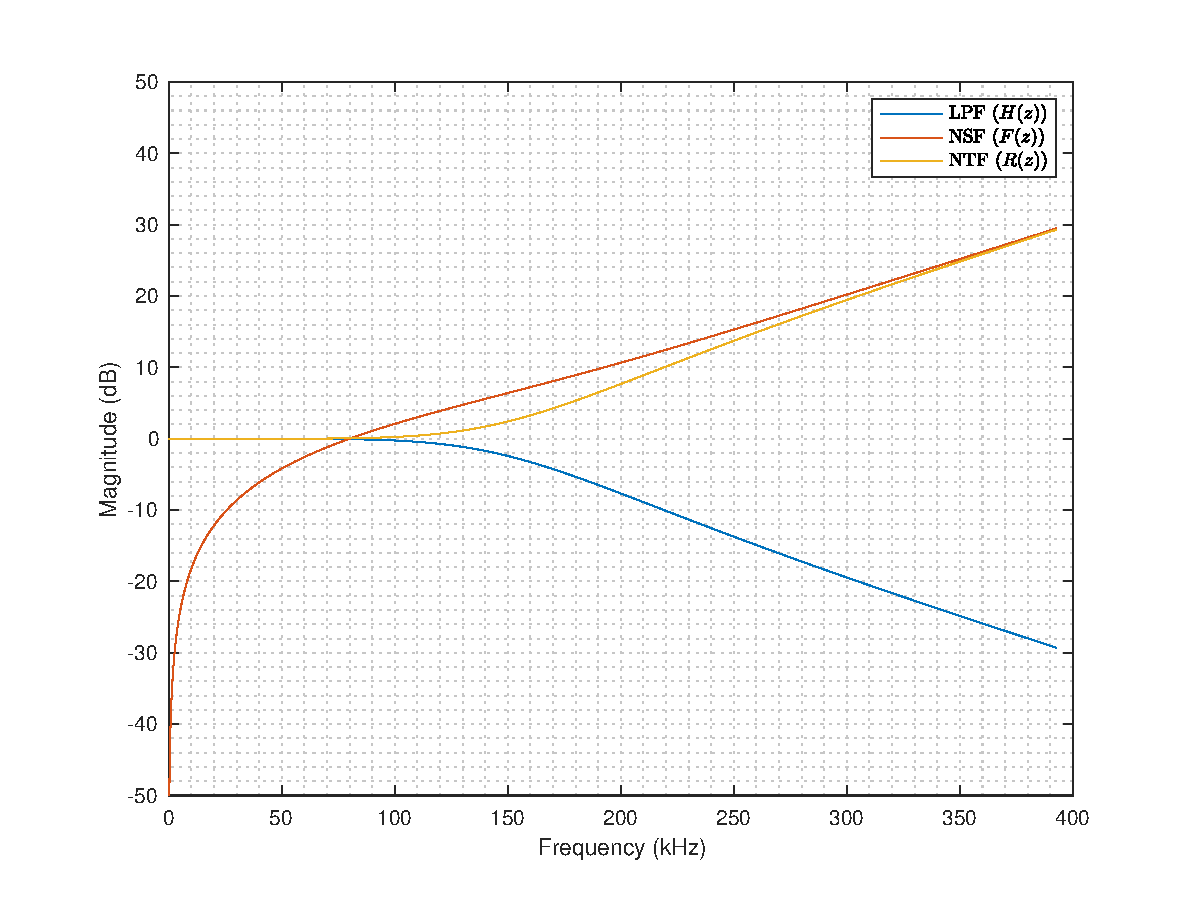
\includegraphics[scale = 0.45]{mat_plots/NO_butter_3_100khz_1Mhz_27_06_2024.eps}
		\caption{Frequency response: Butterworth filter $H(z)$ with $n = 3$ and $F_{c} = 100\mathit{kHz}$ and corresponding noise shaping filter $F(z)$ and noise transfer function $R(z)$.}
        \label{fig:nonoptimal_filter}
	\end{minipage}
	\hfil
	\begin{minipage}{0.45\linewidth}
		\centering
		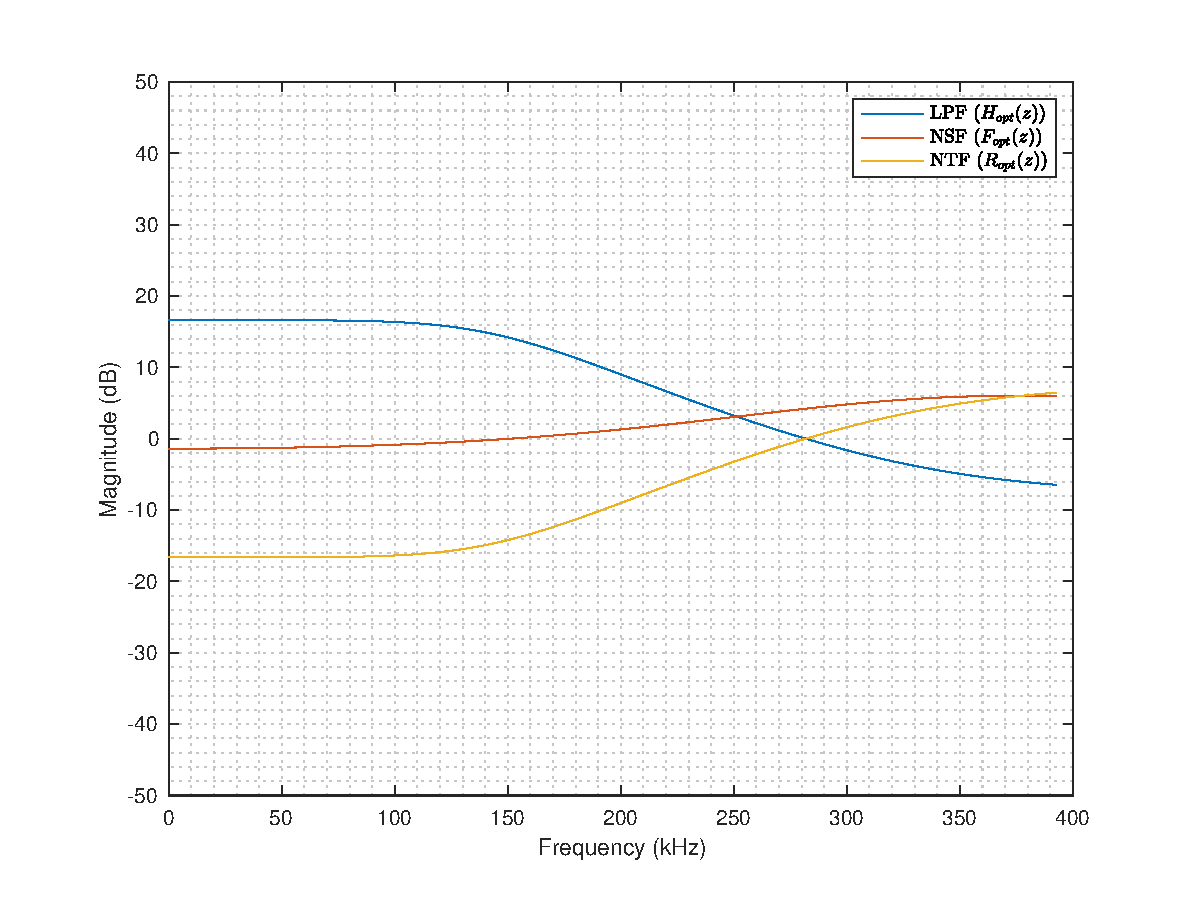
\includegraphics[scale = 0.45]{mat_plots/O_butter_3_100khz_1Mhz_27_06_2024.eps}
		\caption{Frequency response: Optimal noise transfer function $R_{opt}(z)$ for $H(z)$ and corresponding noise shaping filter $F_{opt}(z)$ and low pass filter $H_{opt}(z)$.}
   \label{fig:optimal_filter}
	\end{minipage}
\end{figure}


\begin{table}[!h]
	\caption{ENOB obtained for different methods with uniform quantisation models. Optimal NTF solved for second order butterworth filter with $Fc = 100 \mathit{kHz}$ and $Fs = 1 \mathit{Mhz}$.}
	\centering
	\begin{tabular}{|c|c|c|c|c|c|c|}
	\hline
	ENOB/ Methods & Direct & DSM & NSD (Optimal) & MPC $(N = 1)$ & MPC $(N= 2)$ & MPC $(N= 3)$  \\
        \hline
        6-bit & 6.936 & 8.291 & 9.30  & 9.30 & 9.303 & 9.361\\
        \hline
        8-bit & 9.650 & 10.366 & 11.357  & 11.357 & 11.326 & 11.380\\
         \hline
        12-bit & 13.285 & 14.365 & 15.372  & 15.372 & 15.290 & 15.281\\
	\hline
	16-bit & 17.148 & 18.390 & 19.373  & 19.373 & 19.247& 19.134 \\
	\hline
	\end{tabular}		
\end{table}

\begin{table}[!h]
\caption{ENOB obtained for different methods with nonlinear quantisation models. Optimal NTF solved for second order butterworth filter with $Fc = 100 \mathit{kHz}$ and $Fs = 1 \mathit{Mhz}$.}
	\centering
	\begin{tabular}{|c|c|c|c|c|c|c|}
	\hline
	ENOB/ Methods & Direct & DSM & NSD (Optimal) & MPC $(N = 1)$ & MPC $(N= 2)$ & MPC $(N= 3)$  \\
        \hline
        6-bit &4.177 & 7.977 & 7.022  & 7.022 & 6.99 & 7.007\\
        \hline
        8-bit & 6.526 & 9.968 & 9.228  & 9.228 & 9.251 & 9.241\\
         \hline
        12-bit & 10.830 & 13.679 & 13.524 & 13.524 & 13.503 & 13.509\\
	\hline
	16-bit & 13.577 & 15.77 & 16.156  & 16.156 & 16.157& 16.145 \\
	\hline
	\end{tabular}		
\end{table}
% \subsubsection{PSD of quantised signal}
\begin{figure}[!h]
	\centering
	\begin{minipage}{0.45\linewidth}
		\centering
		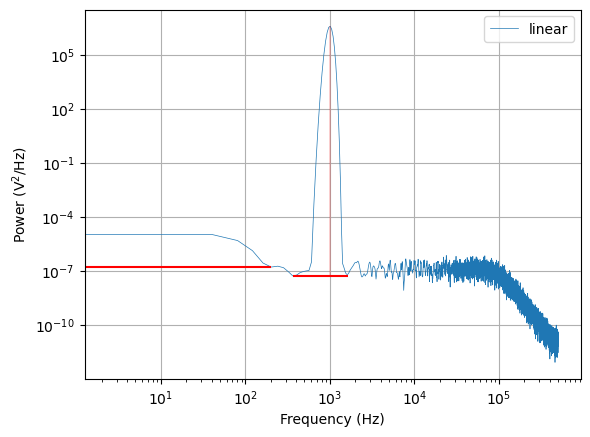
\includegraphics[scale = 0.58]{psd_plots/direct.png}
		\caption{Direct Quantisation}
        \label{fig:direct_psd}
	\end{minipage}
	\hfil
	\begin{minipage}{0.45\linewidth}
		\centering
		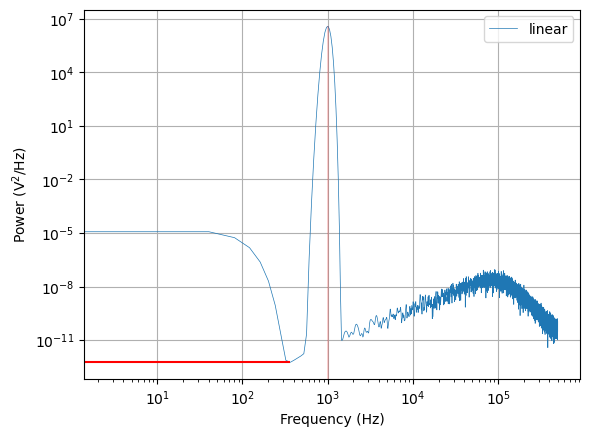
\includegraphics[scale = 0.6]{psd_plots/dsm.png}
		\caption{Delta sigma modulator}
   \label{fig:dsm_psd}
	\end{minipage}
\end{figure}
\begin{figure}[!h]
	\centering
	\begin{minipage}{0.5\linewidth}
		\centering
		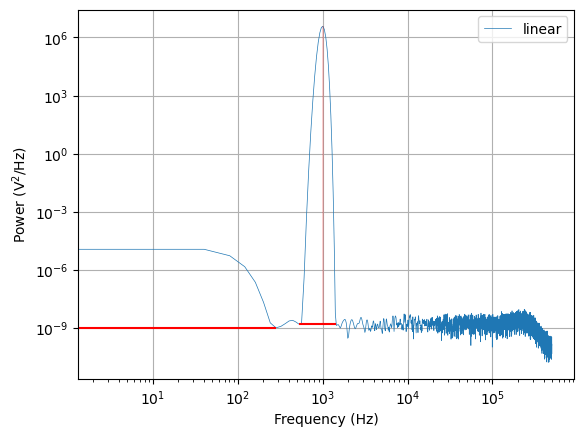
\includegraphics[scale = 0.6]{psd_plots/nsd.png}
		\caption{Noise shaping quantiser}
        \label{fig:nsd_psd}
	\end{minipage}
	\hfil
	\begin{minipage}{0.45\linewidth}
		\centering
		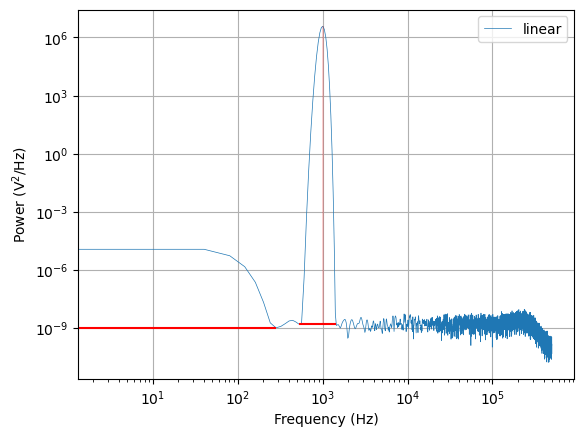
\includegraphics[scale = 0.6]{psd_plots/mpc.png}
		\caption{MPC with optimal noise shaping}
   \label{fig:mpc_psd}
	\end{minipage}
\end{figure}

\subsection{Simulation 2:}
Consider a third order Butterworth filter with $Fc = 100 \mathit{kHz}$ and $Fs = 10 \mathit{Mhz}$.
\begin{table}[!h]
	\caption{ENOB obtained for different methods with nonlinear quantisation models. Optimal NTF solved for second order butterworth filter with $Fc = 100 \mathit{kHz}$ and $Fs = 10 \mathit{Mhz}$.}
	\centering
	\begin{tabular}{|c|c|c|c|c|c|c|}
	\hline
	ENOB/ Methods & Direct & DSM & NSD (Optimal) & MPC $(N = 1)$ & MPC $(N= 2)$ & MPC $(N= 3)$  \\
        \hline
        6-bit &5.041 & 12.355 & 15.576 & 15.576 & 15.548 & 15.577\\
        \hline
        8-bit & 7.392 & 13.950 & 16.988  & 16.988 & 16.406 & 17.008\\
         \hline
        12-bit & 11.210 & 17.368 & 20.952 & 20.952 &  20.950 & 20.931\\
	\hline
	16-bit & 13.877 & 19.413 & 23.369  & 23.369 & 23.372& 23.372 \\
	\hline
	\end{tabular}		
\end{table}


\section{NSD performance: ENOB vs $\gamma_{\eta}$}
\begin{table}[!h]
	\caption{ENOB for different values of $\gamma_{\eta}$}
	\centering
	\begin{tabular}{|c|c|c|c|c|c|c|c|c|c|c|c|c|c|}
	\hline
	 Methods/$\gamma_{\eta}$ & 1.5 & 2 & 3 & 4 &5 & 6 & 7 & 8 & 9 &  10 & 11 & 12  \\
        \hline
        Direct &17.148 & - & - & - & - & - & -& - & - & - & - & - \\
        \hline
        DSM &18.390 & - & - & - & - & - & -& - & - & - & - &  - \\
        \hline
        NSD &19.152 & 19.370 & 19.532 & 19.522 & 19.472 & 19.339 &19.222 & 19.127 & 18.976  & 18.705 & 2.786 & 2.2.458\\
        \hline
        MPC(N=1) &19.152 & 19.370 & 19.532 & 19.522 & 19.472 & 19.339 &19.222 & 19.127 & 18.976  & 18.705 & 2.786 & 2.458\\
         \hline
        MPC(N=2) & 19.098& 19.237 & 19.533 & 19.402 & 19.301 & 19.191 & 19.023 & 18.909 & 18.787 & 18.738 & 18.641 & 18.577\\
	\hline
	MPC(N=3)  & 18.955& 19.133 & 19.266 & 19.180 & 19.040 & 18.868 & 18.746& 18.677 & 18.638 & 18.560 & 18.456 & 18.379\\
 


	\hline
	\end{tabular}		
\end{table}


\begin{table}[!h]
	\caption{ENOB for different values of $\gamma_{\eta}$ using 16 bit DAC.}
	\centering
	\begin{tabular}{|c|c|c|c|c|c|c|c|c|c|c|c|c|c|}
	\hline
	 $\gamma_{\eta}$/ Headroom&0  & 10 & 20 & 30 & 40 &50 & 60 & 70 & 80 & 90  \\
        \hline
        1.5 & 19.152 & 19.066 & 19.004 & 18.924 & 18.830 &18.728 & 18.616 & 18.531 & 18.412 & 18.278  \\
	\hline
	 3 & 19.532 & 19.455 & 19.387 & 19.313 & 19.210 &19.117 & 19.028 & 18.904 & 18.793 & 18.676  \\
	\hline
	 9 & 18.976 & 18.980 & 18.983 & 18.826 & 18.747 &18.640 & 18.527 & 18.429 & 18.314 & 18.187  \\
	 \hline
	 10 & 18.705 & 18.877 &18.807 & 18.728 & 18.637 &18.549 & 18.439 & 18.340 & 18.225 & 18.090  \\
	 \hline
  11 & 2.786 & 18.814 &18.719 & 18.622 & 18.546 &18.457 & 18.341 & 18.245 & 18.129 & 18.00  \\
	 \hline
  12 & 2.458 & 18.700 &18.634 & 18.543 & 18.447 &18.340 & 18.269 & 18.142 & 18.032 & 17.911  \\
	 \hline
   15 & 1.898 & 18.457 &18.366 & 18.285 & 18.192 &18.102 & 18.101 & 17.897 & 17.790 & 17.665  \\
	 \hline
  20 & 1.647 & 18.118 & &  &  & &  & &  &  \\
	 \hline
 30 & 1.398 & 17.602 & &  &  & &  & &  &  \\
	 \hline
   100 & 1.398 & 15.964 & &  &  & &  & &  &  \\
	 \hline
     1000 & 0.828 & 12.642 &12.545& 12.484 &  & &  & &  &  \\
	 \hline
   10000 & 0.826 & 0.631 & 0.495 & 10.318 &10.25  &10.187 & 10.139 & 9.925 & 9.847 & 9.788 \\
	 \hline
	\end{tabular}		
\end{table}


\subsubsection*{Simualtion Results: Binary-MHOQ Formulation}

\begin{table}[!h]
\caption{ENOB obtained for different methods with nonlinear quantisation models. Optimal NTF solved for second order butterworth filter with $Fc = 100 \mathit{kHz}$ and $Fs = 1 \mathit{Mhz}$.}
	\centering
	\begin{tabular}{|c|c|c|c|c|c|c|}
	\hline
	ENOB/ Methods & Direct & DSM & NSD (Optimal) & MPC $(N = 1)$ [Time (s)] & MPC $(N= 2)$[Time (s)] & MPC $(N= 3)$  \\
        \hline
        6-bit (BINARY) & 6.693 & 8.322 & 9.051  & 9.051 [$\approx 880$ s] & 9.135 [$\approx 3820$ s] & - \\
        \hline
        6-bit (SCALED) & 6.693 & 8.322 & 9.051  & 9.051 [$\approx 120$ s] & 9.093 [$\approx 380$ s]&  9.141 [$\approx 450$ s]\\
         \hline
	\end{tabular}		
\end{table}

\section{Switching Frequency Minimization}
The optimization problem \eqref{eq:optobj1}-\eqref{eq:optconst3} can be reformulated as an optimization problem with the binary variables. Let $\mathcal{B}$ be the number of bits.  $b_{i} = \{0,1\}$ and $Q_{i}$ $, i = \{0, 1, \ldots, 2^{\mathcal{B}}-1\}$, be the binary variables and quantisation levels, respectively. 
\begin{align}
		& y^{\ast}(t) = \arg  \min_{y(t) }	V_{N}  = \sum_{t=k}^{k+N-1} e^{2}(t) + \beta \mathcal{N}_{s}\label{eq:optobj121}\\
		\intertext{subject to}
		&x(t+1) = A x(t) + B (w(t)-y(t))	\label{eq:optconst122}	\\
		&e(t) = Cx(t) + (w(t)-y(t))	\label{eq:optconst223}	\\
		&y(t) = \sum_{i = 0}^{2^{\mathcal{B}}-1} Q_{i}b_{i}(t), \quad \sum_{i = 0}^{2^{\mathcal{B}}-1}b_{i}(t)  =1, \quad b_{i} = \{0,1\}. \label{eq:optconst324} \\
		&\mathcal{N}_{s} = \sum_{i = 0}^{2^{\mathcal{B}-1}} |b_{i}(t) - b_{i}(t-1)|
	\end{align}
	where $b_{t-1}$ is the state of the switch $i$ at the previous sampling period and $b_{i}(t)$ is the sate of switch $i$ at the current state and $\beta$ is the weighting factor. 

\section{Closed Form Solution:}
Let $N$ be the prediction horizon of the moving horizon implementation and $\mathbb{U}$ the quantisation levels. The $N$th power cartesian product of the set $\mathbb{U}$ for $N$ is defined as  $\mathbb{U}^{N}:= \mathbb{U} \ldots \times \ldots \mathbb{U}$. Let $n_{\mathbb{U}}$ represent the number of element in the set $\mathbb{U}$ i.e., number of quantisation levels, then the number of elements on the set $\mathbb{U}^{N}$ is $n_{\mathbb{U}}^{N}$. Also, let $v_{i}, i = \{1, 2, \ldots, n_{\mathbb{U}}^{N}\}$ represent the elements of the set $\mathbb{U}^{N}$. Then, the closed form solution of the moving horizon implementation of the optimisation problem \eqref{eq:optobj1}-\eqref{eq:optconst3} is 
\begin{equation}
	\mathbf{y}^{\ast}(k) = \Psi^{-1} q_{\tilde{\mathbb{U}}^{N}} \big[\Psi \mathbf{w}(k) + \Gamma x(k)\big]
\end{equation}
where 
\begin{align*}
\mathbf{y}^{\ast}(k) = \begin{bmatrix}
	y(k) \\ y(k+1) \\ \vdots \\ y(k+N-1)
\end{bmatrix},
\quad
\mathbf{w}(k) = \begin{bmatrix}
	w(k) \\ w(k+1) \\ \vdots \\ w(k+N-1)
\end{bmatrix},
\quad
\Gamma = \begin{bmatrix}
	C \\ CA \\ \vdots \\ CA^{N-1}
\end{bmatrix},
\quad
\Psi = \begin{bmatrix}
	h_{0} & 0 & \cdots & 0 \\
	h_{1} & h_{0} & \ddots & \vdots \\
	\vdots & \ddots & \ddots & 0 \\
	h_{N-1} & \ldots & h_{1} & h_{0}
\end{bmatrix},
\end{align*}
and $q_{\tilde{\mathbb{U}}^{N}}[.]$ represent the nearest neighbor vector quantisation (direct quantisation) and image of this mapping is the set 
\begin{eqnarray*}
	\tilde{\mathbb{U}}^{N} := \{\tilde{v}_{1}, \tilde{v}_{2}, \ldots, \tilde{v}_{r}\} \subset \mathbb{R}^{N}, \qquad r = n_{\mathbb{U}}^{N},
\end{eqnarray*}
with $\tilde{v}_{i} = \Psi v_{i}$ and $v_{i} \in \mathbb{U}^{N} = \{ v_{1}, v_{2}, \ldots, v_{n_{\mathbb{U}}}\}$. The elements of the matrices $\Psi$, $\{h_{0}, h_{1}, \ldots, h_{N-1}\}$ are the impulse response of the filter $H(z) = 1 + C(zI-A)^{-1}B$ and  $h_{0}=1$.


The moving horizon implementation of the above solution is 
\begin{equation}
	{y}(k) =[1, 0, \ldots, 0]\mathbf{y}^{\ast}(k) = [1, 0, \ldots, 0] \Psi^{-1} q_{\tilde{\mathbb{U}}^{N}} \big[\Psi \mathbf{w}(k) + \Gamma x(k)\big].
\end{equation}
Replacing $x(k) = (zI- A)^{-1}B (a(k) - u(k))$ and with further manipulation, we get, 
\begin{equation}
	{y}(k) =[1, 0, \ldots, 0] \Psi^{-1} q_{\tilde{\mathbb{U}}^{N}} \big[\Psi \bigl\{ \mathcal{H}(z)  \mathbf{w}(k) - \big[ \mathcal{H}(z) -I\big] \mathbf{y}^{\ast}(k)\bigr\} \big].
\end{equation}
where 
\begin{equation}
	\mathcal{H}(z) = \begin{bmatrix}
		1 + \mathcal{H}_{1}^{\prime}(z)	 & 0 &\ldots & \ldots & 0 \\
		\mathcal{H}_{2}^{\prime}(z)	 & 1 & 0 & \ldots & 0 \\
		\mathcal{H}_{3}^{\prime}(z)	 & 0 & 1 & \ldots & 0 \\
		\vdots & \vdots & \ddots & \ddots & \vdots \\
		\mathcal{H}_{N}^{\prime}(z)	 & 0 & 0 & \ldots & 1 \\
	\end{bmatrix}	
	\quad
	\textrm{and}
	\quad
\mathcal{H}_{i}^{\prime}(z) = \big[\Psi^{-1}\big]_{i,\ast} \Gamma(zI- A)^{-1}B
\end{equation}
and $ \big[\Psi^{-1}\big]_{i,\ast}$ denotes the $i$ th row of $\Psi^{-1}$.

\subsection{ Prediction horizon $N = 1$:}
When the prediction horizon is $N = 1$, $\Psi = 1$ since $h_{0}=1$ and  
\begin{align*}
\mathcal{H}(z) = 1 + \mathcal{H}_{1}^{\prime}(z) = 1 + C(zI- A)^{-1}B = H(z)
\end{align*}
and the moving horizon implementation is 
\begin{equation}
	{y}(k) =  q_{\tilde{\mathbb{U}}^{N}} \big[{H}(z)  {w}(k) - \big[ {H}(z) -I\big] {y}^{\ast}(k)\big].
\end{equation}
and $ q_{\tilde{\mathbb{U}}^{N}}[.] = q_{{\mathbb{U}}^{N}}[.]$ for $\Psi = 1$ and it becomes scalar (direct) quantisation.

\begin{figure}[!h]
	\centering
	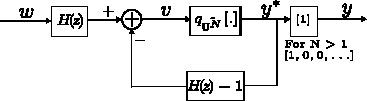
\includegraphics[scale = 2]{figures/nsd_mhoq_implementation.pdf}
	\caption{NSD equivalent of MHOQ implementation for $N=1$.}
	\label{fig:nsd_mhoq_implementation}
\end{figure}
\subsection{Prediction horizon $N=2$:}
When the prediction horizon is $N = 1$, $\Psi = \begin{bmatrix}
h_{0} & 0 \\ h_{1} & h_{0}
\end{bmatrix}$ and thus  $\Psi^{-1} = \frac{1}{h_{0}^{2}} \begin{bmatrix} h_{0} & - h_{1} \\ 0 & h_{0} \end{bmatrix}  = \begin{bmatrix} 1 & - h_{1} \\ 0 & 1 \end{bmatrix}$ since $h_{0} = 1$. We get, 
\begin{align*}
	\mathcal{H}_{1}^{\prime}(z) &=  \begin{bmatrix}
		1 & -h1
	\end{bmatrix} \Gamma(zI- A)^{-1}B = (C - h_{1}CA) (zI- A)^{-1}B =H(z)  - h_{1}CA(zI- A)^{-1}B -1 \\
	\mathcal{H}_{2}^{\prime}(z) &=  \begin{bmatrix}
		0 & h_{0}
	\end{bmatrix} \Gamma(zI- A)^{-1}B = CA(zI- A)^{-1}B
\end{align*}


Then

\begin{align*}
\mathcal{H}(z) = \begin{bmatrix}
1 + \mathcal{H}_{1}^{\prime}(z) & 0\\
 \mathcal{H}_{2}^{\prime}(z) &1
\end{bmatrix} = \begin{bmatrix}	
1 + \mathcal{H}_{1}^{\prime}(z) & 0\\
 \mathcal{H}_{2}^{\prime}(z) &1
\end{bmatrix} = \begin{bmatrix}
	H(z)  - h_{1}CA(zI- A)^{-1}B & 0  \\
CA(zI- A)^{-1}B & 1
\end{bmatrix}
\end{align*}
and the moving horizon implementation is 
\begin{align*}
	{y}(k)  &=[1, 0] \Psi^{-1} q_{\tilde{\mathbb{U}}^{N}} \big[\Psi \bigl\{ \mathcal{H}(z)  \mathbf{w}(k) - \big[ \mathcal{H}(z) -I\big] \mathbf{y}^{\ast}(k)\bigr\} \big] \\
&=[1, 0] \Psi^{-1} q_{\tilde{\mathbb{U}}^{N}} \big[\Psi  \mathcal{H}(z)  \mathbf{w}(k) - \Psi  \big[ \mathcal{H}(z) -I\big] \mathbf{y}^{\ast}(k) \big] \\
&=[1, 0] \Psi^{-1} q_{\tilde{\mathbb{U}}^{N}} \big[\Psi  \mathcal{H}(z) \big( \mathbf{w}(k) - \mathbf{y}^{\ast}(k) \big) + \Psi  \mathbf{y}^{\ast}(k) \big] \\
&=[1, 0] \Psi^{-1} q_{\tilde{\mathbb{U}}^{N}} \Bigg[ \begin{bmatrix}
H(z) - h_{1}CA(zI-A)^{-1}B & 0 \\ h_{1} H(z) - (h_{1}^{2} - 1) CA (zI-A)^{-1} B & 1
\end{bmatrix} \mathbf{w}(k)- \begin{bmatrix}
  H(z) - 1 - h_{1}CA(zI-A)^{-1}B  & 0 \\  h_{1} ( H(z) - 1)  - (h_{1}^{2} - 1) CA (zI-A)^{-1} B  & 0
\end{bmatrix} \mathbf{y}^{\ast}(k) \Bigg] \\
&=[1, 0] \Psi^{-1} q_{\tilde{\mathbb{U}}^{N}} \Bigg[ \begin{bmatrix} H(z) & 0 \\ 0 & 0 \end{bmatrix} \mathbf{w}(k) - \begin{bmatrix} H(z) -1 & 0 \\ 0 & 0 
\end{bmatrix} \mathbf{y}^{\ast}(k) \\ &+ \begin{bmatrix} 
 - h_{1}CA(zI-A)^{-1}B & 0 \\ h_{1} H(z) - (h_{1}^{2} - 1) CA (zI-A)^{-1} B & 1
\end{bmatrix} \mathbf{w}(k)- \begin{bmatrix}
  - h_{1}CA(zI-A)^{-1}B  & 0 \\  h_{1} ( H(z) - 1)  - (h_{1}^{2} - 1) CA (zI-A)^{-1} B  & 0
\end{bmatrix} \mathbf{y}^{\ast}(k) \Bigg]
\end{align*}

\begin{figure}[!h]
	\centering
	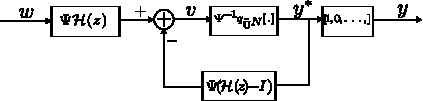
\includegraphics[scale = 2]{figures/nsd_mhoq_implementation_N2.pdf}
	\caption{NSD equivalent of MHOQ implementation for $N>2$.}
	\label{fig:nsd_mhoq_implementation_N2}
\end{figure}


% \begin{figure}[!h]
% 	\centering
% 	\begin{minipage}{0.45\linewidth}
% 		\centering
% 		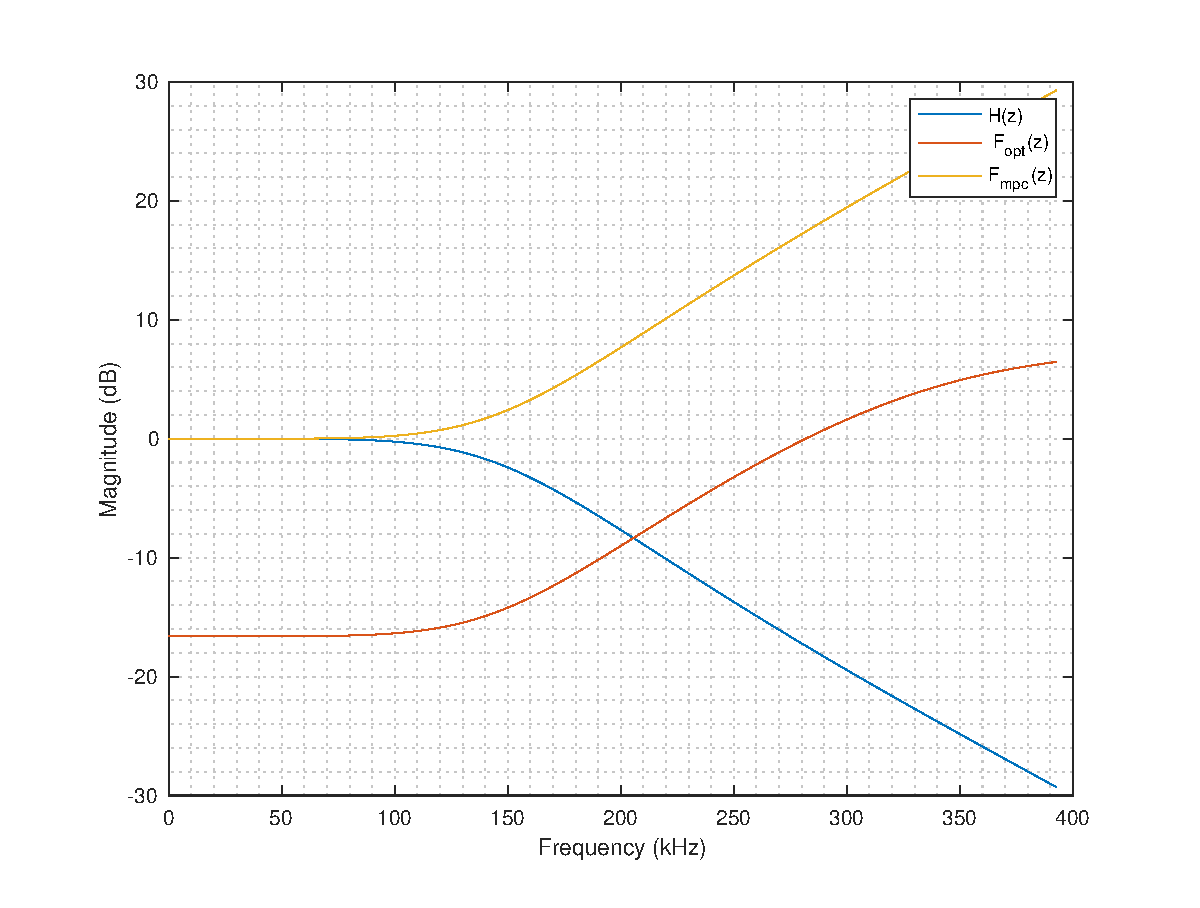
\includegraphics[scale = 0.45]{mat_plots/butter_3_100khz_1Mhz_1.eps}
% 		\caption{Frequency response: Butterworth filter with $n = 3$ and $F_{c} = 100\mathit{kHz}$ and corresponding optimal noise shaping filter and low pass filter}
%         \label{fig:nonoptimal_filter}
% 	\end{minipage}
% 	\hfil
% 	\begin{minipage}{0.45\linewidth}
% 		\centering
% 		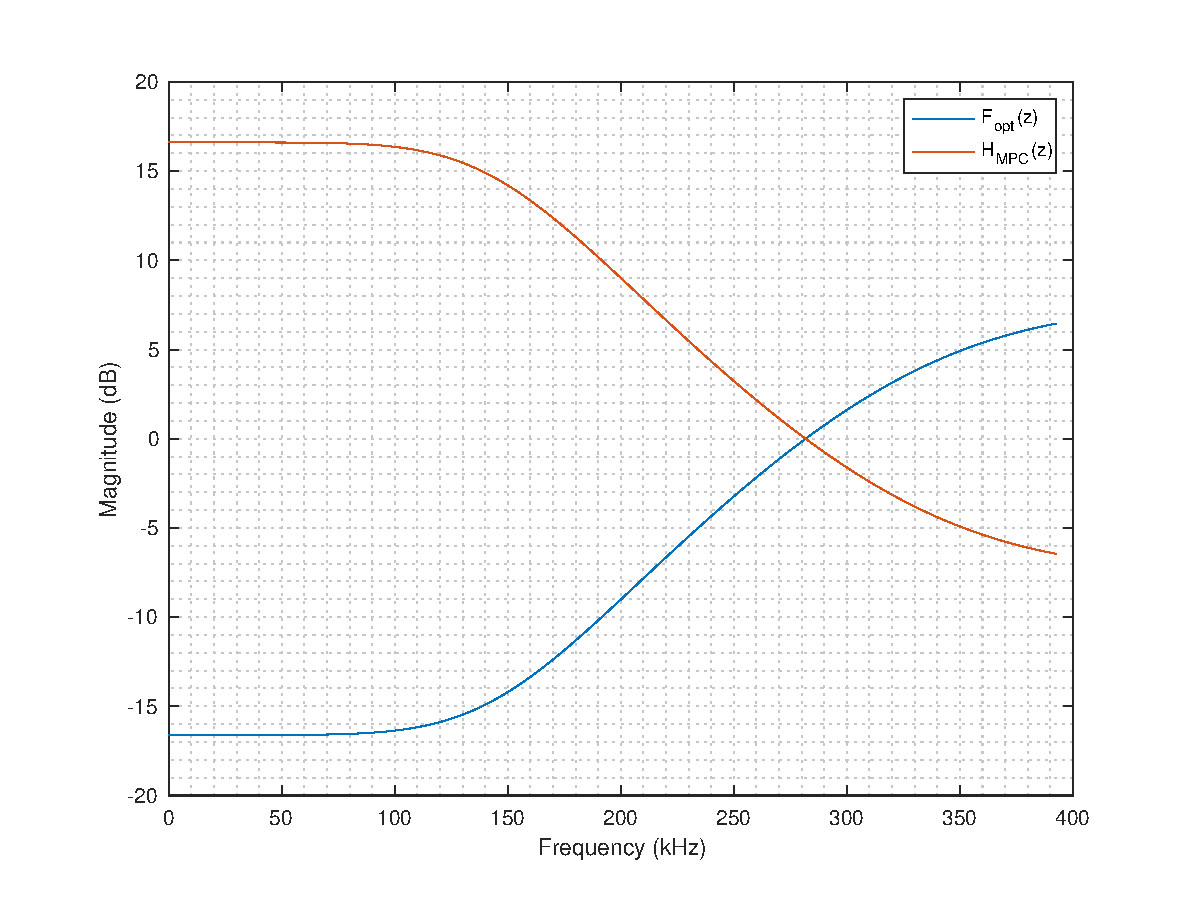
\includegraphics[scale = 0.45]{mat_plots/butter_3_100khz_1Mhz_2.eps}
% 		\caption{Frequency response: Optimal noise shaping filter and corresponding low pass filter}
%    \label{fig:optimal_filter}
% 	\end{minipage}
% \end{figure}

\newpage
%\section{References}
%\label{sec:org89add8d}
\bibliographystyle{unsrt}
\bibliography{references_new} 

\section{Scribble}

We want to minimise this error: $\bar{e} = H y - H w = H v + H \epsilon - H w$

$\bar{e} = H y - H w = H v + H \epsilon - H w$

What is $\bar{e}$ when
\begin{itemize}
    \item the feedback filter is a (double) delay (standard delta-sigma)
    \item the feedback filter is optimal
    \item the feedback filter is implemented in the MPC formulation with horizon length 1, 2, 3, ...
\end{itemize}
Things to study
\begin{itemize}
    \item[done] Need to handle saturation (no need as optimal gain appears to be 3)
    \item[done] What happens when there is a constant noise floor, unaffected by the noise-shaping (no need as small headroom is sufficient for gain of 3)
    \item Can we limit the rate
    \item Adding in INL
\end{itemize}

Total noise and distortion:
$$
\sigma_t = \sigma_n + \sigma_q
$$

$$
\frac{\sigma_s}{\sigma_n + \sigma_q}
$$
\end{document}